\documentclass[a4paper,10pt,titlepage]{article}
\usepackage[utf8]{inputenc}
\usepackage{lmodern}
\usepackage{microtype}

\usepackage[backend=biber]{biblatex}
\bibliography{solutions_bibliography}
% \usepackage{fancyhdr}
% \pagestyle{fancy}


\usepackage[dvipsnames]{xcolor}
\usepackage{amsmath}
\usepackage{amssymb}
\usepackage{gensymb}
\usepackage{multicol}
\usepackage{amsthm}
\usepackage{adjustbox}
\usepackage[hidelinks]{hyperref}
\usepackage{cleveref}
\usepackage{pgfplots}
\pgfplotsset{compat=1.11}
\usepackage{graphicx}
\usepackage{sidecap}
\sidecaptionvpos{figure}{c}
\usepackage{float}
\usepackage{eufrak}
\usepackage{polynom}
\usepackage{caption}
\usepackage{commath}
\usepackage{titlepic}

\usepackage{flafter}

\usepackage[margin=1in]{geometry}
\usepackage{changepage}
\usepackage{titlesec}
\titleformat{\section}{\normalfont\Large\bfseries\centering}{Section~\thesection:}{1em}{}

\newtheorem*{thm}{Theorem}
\newtheorem*{iden}{Identity}
\theoremstyle{definition}
\newtheorem*{defn}{Definition}
\DeclareMathOperator{\cis}{cis}
\DeclareMathOperator{\proj}{proj}
\DeclareMathOperator{\carg}{arg}
\newcommand*\realp[1]{ \mathfrak{Re} \left ( {#1} \right )  }
\newcommand*\imagp[1]{ \mathfrak{Im} \left ( {#1} \right )  }

\begingroup
    \makeatletter
    \@for\theoremstyle:=definition,remark,plain\do{%
        \expandafter\g@addto@macro\csname th@\theoremstyle\endcsname{%
            \addtolength\thm@preskip\parskip
            }%
        }
\endgroup

\usepackage[inline]{enumitem}

\def\signed #1{{\leavevmode\unskip\nobreak\hfil\penalty50\hskip2em
  \hbox{}\nobreak\hfil(#1)%
  \parfillskip=0pt \finalhyphendemerits=0 \endgraf}}

\newsavebox\mybox
\newenvironment{aquote}[1]
  {\savebox\mybox{#1}\begin{quote}}
  {\signed{\usebox\mybox}\end{quote}}
\newcommand{\hard}{\refstepcounter{enumi}\item[$^\star$\theenumi.]}
\newcommand{\harder}{\refstepcounter{enumi}\item[$^{\star\star}$\theenumi.]}
\newcommand{\ditem}{\refstepcounter{enumi}\item[$^{\dagger}$\theenumi.]}
\newcommand{\dhard}{\refstepcounter{enumi}\item[$^{\dagger\star}$\theenumi.]}
\newcommand{\dharder}{\refstepcounter{enumi}\item[$^{\dagger\star\star}$\theenumi.]}
% \newcommand{\hard}{\item}
% \newcommand{\harder}{\item}

\usepackage[english]{babel}
\usepackage[autostyle, english = british]{csquotes}
\MakeOuterQuote{"}

\title{\textbf{\textit{Solutions}}}
\author{Alex Elzenaar}%\\Upper Hutt College}
\date{\today}
\titlepic{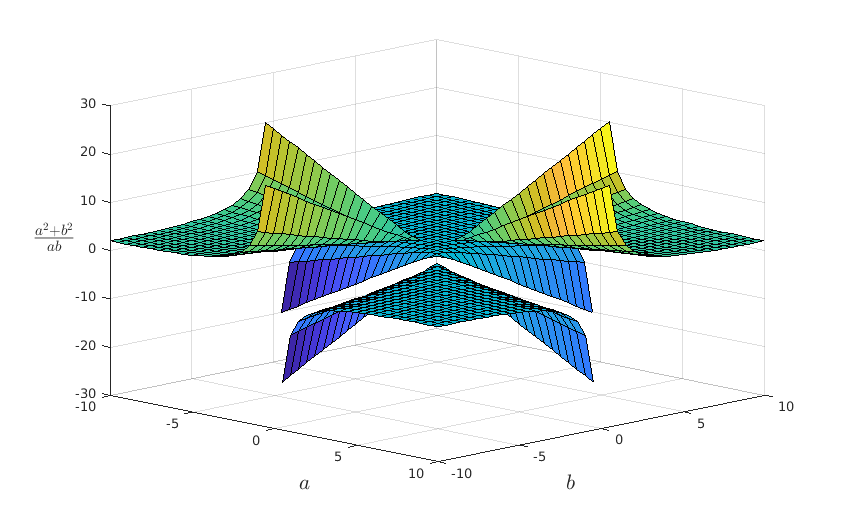
\includegraphics[width=\textwidth]{problem.png}}

% \makeatletter
% \let\runauthor\@author
% \renewcommand{\rightmark}{\runauthor}
% \makeatother

\begin{document}

\setcounter{tocdepth}{1}
\maketitle
\newpage\null\thispagestyle{empty}\newpage
\pagenumbering{arabic}

\tableofcontents

\titleformat{\section}{\clearpage\titlerule[0.8pt]\vspace{0.5ex}\normalfont\Large\bfseries\centering}{Section~\thesection:}{1em}{}[{\titlerule[0.8pt]}]
\let\oldsection\section
\renewcommand\section{\clearpage\oldsection}

\section{Introduction}\label{sec:intro}
What does it really mean to \emph{solve} an equation? These notes attempt
to briefly present an outline to Level 3 and Scholarship methods for both finding
solutions to equations and interpreting those solutions.

We will begin with simple linear equations, and will work our way up to arbitrary
polynomials. Geometric and algebraic interpretations will be presented, along with
a number of examples and exercises.

Philosophically, we have made the decision to leave a number of important results
(chiefly de~Moirve's theorem) as exercises. However, these results are required
knowledge for the later problems --- so the reader should at least glance at previous
problems before attempting later ones.

Some exercises are much more difficult than others, and the difficulty does not
always increase within a section (i.e. sometimes the first exercises can be quite
hard). The number of stars by each problem is roughly indicative of a mixture of
difficulty and time required. There is, however, no guarantee that the author's
idea of a difficult question will match up with the reader's idea of a difficult
question!

Note that there are fully worked answers for all problems, and often these solutions
contain insights or additional information not in the main text. They are designed to
be read in conjunction with the problems (but have a go yourself before reading the
solutions). Additional information on the problems themselves, as well as a discussion
of some notation, can be found in the introduction to the solutions.

The culmination of the text comes in sections \ref{sec:roots} and \ref{sec:cubic}; the former is a digression
into more pure mathematics (developing a theory of the roots of unity), and the latter
is a more applied section (developing the solution of the general cubic). Both should
be easily within reach of the enthusiastic student. The section on geometry, \ref{sec:geometry}, also includes
a selection of material beyond that needed for level 3.

\section{Quadratic Equations}\label{sec:quadratic}
\begin{figure}
  \centering
  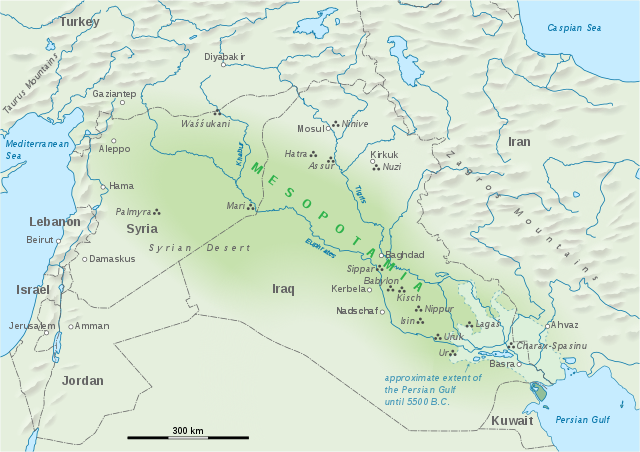
\includegraphics[width=0.8\textwidth]{meso}
  \caption[blag]{Babylon in ancient Mesopotamia.\footnotemark\label{fig:babylon2}}
\end{figure}
\footnotetext{By Goran tek-en - Own work. Based on: Karte von Mesopotamien, Mesopotamia Syria. CC BY-SA 3.0, \url{https://commons.wikimedia.org/w/index.php?curid=30851043}}

Even earlier than the Greeks, mathematics was being done in ancient Babylon.
Several ancient clay tablets from the Old Babylonian period (between 1800 and 1600 BCE)
contain mathematical problems and solutions. Such a problem, given on the tablet
illustrated in \cref{fig:babylon2}, is (translated of course):\footnote{~Translation from \cite{Ste08}.}

\begin{quote}
  I have added up seven times the side of my square and eleven times the area,
  getting 6;15.
\end{quote}

\begin{figure}\label{fig:babylon2}
  \centering
  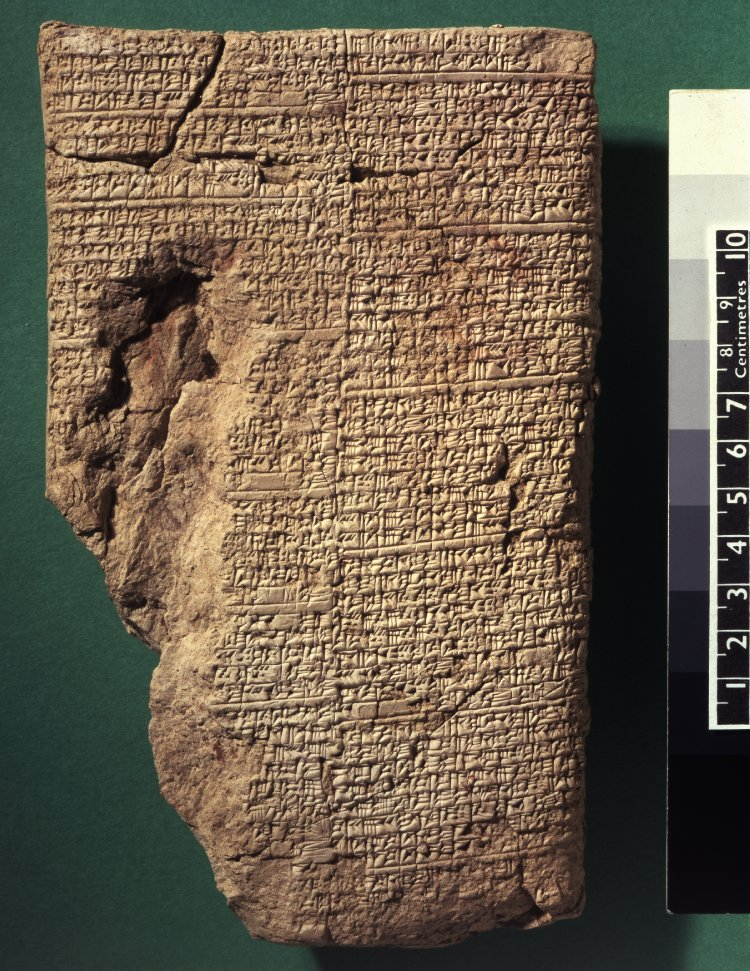
\includegraphics[width=\textwidth]{babylon2}
  \caption[blag]{Tablet BM 13901; image from the British Museum.}
\end{figure}

The number 6;15 is in sexagesimal notation; it means $ 6 + \frac{15}{60} = 6.25 $. We
can therefore rewrite this problem as follows, where $ x $ is the length of the side
of the square and $ x^2 $ is the area:
\begin{displaymath}
  11x^2 + 7x = 6.25
\end{displaymath}
Rearranging this we have $ 11x^2 + 7x - 6.25 = 0 $, and so we see that our problem is simply
to find the $ y$-intercepts of a parabola, graphed as \cref{fig:parabola1}. We find that the
only positive solution to the equation is $ x = 0.5 $ --- or 0;30 in Babylonian notation.

\begin{figure}
  \centering
  \begin{tikzpicture}
    \begin{axis}[
      xlabel=$x$,
      ylabel=$y$,
      axis lines=middle,
      height=7cm
    ]
      \addplot[domain=-1:1, samples=100, color=purple]{11*x^2 + 7*x - 6.25};
    \end{axis}
  \end{tikzpicture}
  \caption{The graph of $ y = 11x^2 + 7x - 6.25 $.\label{fig:parabola1}}
\end{figure}

This problem is an example of a quadratic equation --- an equation where the highest
power of $ x $ is 2. All quadratic equations can be put into the form $ ax^2 + bx + c = 0 $,
where $ a $, $ b $, and $ c $ are constants.

All of the equations which we will consider this year can be put into the form $ f(x) = 0 $ for
some function $ f $. The values $ x $ which satisfy the equation are called \emph{solutions} of
the equation, or \emph{roots} or \emph{zeroes} of the function.

\subsection*{The Quadratic Formula}
In fact, there is a general formula to solve \emph{any} quadratic equation. The
following proof of this illustrates the idea of \emph{completing the square}, which
is a way to reduce the difficult problem of solving a general quadratic equation to a simpler
problem: that of solving $ y^2 = m $ for $ y $ given a value for $ m $. A second
proof is given as an exercise at the end of the section.

\begin{thm}[Quadratic Formula]
  A quadratic equation $ ax^2 + bx + c = 0 $ (where $ a \neq 0 $) has at most
  two solutions, which are given by
  \begin{displaymath}
    x = \frac{-b \pm \sqrt{b^2 - 4ac}}{2a}.
  \end{displaymath}
\end{thm}

\begin{proof}
  We want to transform our equation so that it looks like $ (\cdots)^2 = d $; then we can just take the square root of both sides and
  solve. Let us na\"ively guess that the bracket will look like $ a(x + b/2a)^2 $. If we expand this, we have
  \begin{displaymath}
    a\left(x + \frac{b}{2a}\right)^2 = ax^2 + bx + \frac{b^2}{4a}.
  \end{displaymath}
  Comparing with our original equation, we are almost there: if we add on the constant term $ c - \frac{b^2}{4a} $, all the unwanted
  material vanishes and we are left with the correct expression. With a little bit of manipulation, we obtain the required explicit
  formula for the solutions:
  \begin{gather*}
    0 = ax^2 + bx + c = a\left(x + \frac{b}{2a}\right)^2 + c - \frac{b^2}{4a}\\
    \frac{b^2}{4a} + c = a\left(x + \frac{b}{2a}\right)^2\\
    \pm\sqrt{\frac{b^2}{4a^2} + \frac{c}{a}} - \frac{b}{2a} = x\\
    \frac{-b \pm \sqrt{b^2 - 4ac}}{2a} = x.
  \end{gather*}
\end{proof}

The expression $ b^2 - 4ac = \Delta_2 $ is known as the \textit{discriminant} of the
quadratic, and it determines the nature of the solutions; if $ \Delta_2 = 0 $, there is
one repeated root, while if $ \Delta_2 > 0 $ there are two real roots. We discuss the case
where $ \Delta_2 < 0 $ later on.

\subsection*{Factors}
To create a quadratic equation with given solutions, we write down a linear expression
for each solution that evaluates to zero when the solution is substituted in, and then multiply
them. For example, if we wanted a quadratic equation with the solutions $ x = 2 $ and $ x = 3 $,
we take the two expressions $ x - 2 $ and $ x - 3 $, multiply the left hand sides together
(obtaining $ (x-2)(x-3) = x^2 - 5x + 6 $), and set it to zero.

This works because if we substitute in one of our original solutions (in our
example, 2 or 3) then one of the two parts of the left hand side will become zero
and so the entire left hand side becomes zero.

In general, this idea works for higher-degree equations (like cubics, quartics,
and so on). We can make a cubic with the solutions $ x = -3 $, $ x = 9 $, and
$ x = 13 $ by writing $ 0 = (x+3)(x-9)(x-13) $.

We can even multiply together higher-degree polynomials to create a polynomial
that has the roots of all of them --- if (for example) we take the equation
$ (x^2 - 4)(x^2 - 9) = 0 $, it will have the four solutions $ x = \pm 2 $ and $ x = \pm 3 $.

The polynomials which multiply together together to form a larger polynomial are known
as \textit{factors} of the larger polynomial, and the process of splitting a polynomial
into factors is known as \textit{factorising}.

\begin{figure}
  \centering
  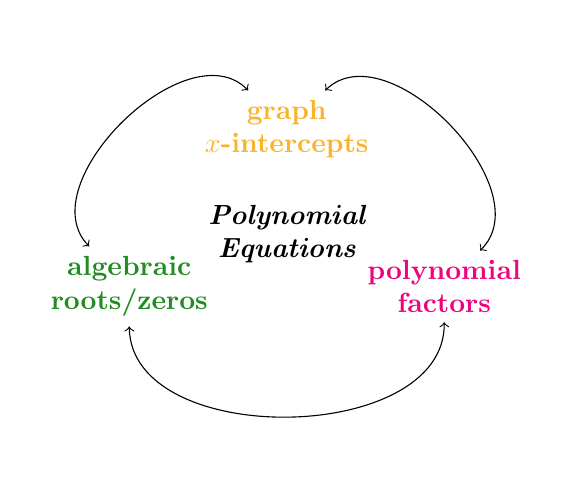
\begin{tikzpicture}
    \node (A) at (-2,0) {\color{ForestGreen}\textbf{\shortstack{algebraic\\roots/zeros}}};
    \node (B) at (0,2) {\color{Dandelion}\textbf{\shortstack{graph\\$ x $-intercepts}}};
    \node (C) at (2,0) {\color{RubineRed}\textbf{\shortstack{polynomial\\factors}}};
    \node () at (0,0.67) {\textbf{\textit{\shortstack{Polynomial\\Equations}}}};

    \draw (A) edge[<->,bend left=90] (B);
    \draw (B) edge[<->,bend left=90] (C);
    \draw (C) edge[<->,bend left=90] (A);
  \end{tikzpicture}
  \caption{Relationships between concepts.}
\end{figure}

\subsection*{Exercises}
\begin{enumerate}
  \item Find an example of a \textbf{quadratic equation} with the solutions:
        \begin{enumerate*}
          \item $ x = 7 $ and $ x = 4 $,
          \item $ x = 7 $ and $ x = -4 $,
          \item $ x = -7 $ and $ x = -4 $, and
          \item the single solution $ x = 3 $.
        \end{enumerate*}
  \item Use the discriminant $ \Delta_2 $ of the following quadratics to find the
        number of distinct real roots each one has, without explicitly calulating
        those roots.
        \begin{multicols}{2}
        \begin{enumerate}
          \item $ 3x^2 + 6x + 3 = 0 $
          \item $ x^2 + 10x + 1 = 0 $
          \item $ x^2 + 5x + 9 = 0 $
          \item $ x^2 - \frac{14x}{3} + \frac{49}{9} = 0 $
        \end{enumerate}
        \end{multicols}
  \item Use the \emph{difference of two squares} identity $ x^2 - b^2 = (x-b)(x+b) $ to factorise and hence
        solve the following equations for $ x $:
        \begin{multicols}{2}
        \begin{enumerate}
          \item $ x^2 - 9 = 0 $
          \item $ x^2 - 7 = 0 $
          \item $ x^2 - 15 = 1 $
          \item $ x^2 - 2ab = a^2 + b^2 $
        \end{enumerate}
        \end{multicols}
  \hard Prove that $ ax^2 + bx + c = Ax^2 + Bx + C $ implies that $ a = A $, $ b = B $, and $ c = C $.
        This result allows us to \textit{match coefficients}, an important tool which we can use to
        reason about the symmetries of polynomials.
  \item Show that if $ \alpha $ and $ \beta $ are the two solutions of $ x^2 + bx + c = 0 $, then
        we have $ -b = \alpha + \beta $ and $ c = \alpha\beta $.
  \item Factorise $ x^2 - 3x - 40 $ by inspecting the coefficients and using the
        identity that a quadratic with the two solutions $ a $ and $ b $ is given
        by $ (x-a)(x-b) = x^2 -(a+b)x + ab $ (note the change of sign in the factors).
  \item For which values of $ k $ does the graph of the quadratic function
        $ y = x^2 +(3k-1)x + (2k+10) $ not touch the $ x$-axis?
  \item Do the zeroes of a function uniquely identify that function? Why/why not?
  \hard Solve the following equations in the real numbers:
        \begin{enumerate*}
          \item $ w^4 + 30w^2 + 29 = 0 $, and
          \item $ 3 e^{2x} - 24 e^x - 8 = 0 $.
        \end{enumerate*}
  \item Write each of the following in the form $ (x + p)^2 = q $ for some $ p $ and $ q $, and hence find their
        solutions by completing the square.
        \begin{multicols}{2}
        \begin{enumerate}
          \item $ x^2 - 3x + 4 = 0 $
          \item $ x^2 - 6x - 10 = 0 $
          \item $ x^2 - 26x + 47 = 0 $
          \item $ 6x^2 - 12x + 13 = 0 $
          \item $ -2x^2 + 3x + 5 = 0 $
        \end{enumerate}
        \end{multicols}
  \item Suppose that $ x^2 + bx + c = 0 $ has two roots, $ \alpha $ and $ \beta $.
        \begin{enumerate}
          \item Show that $ \alpha^2 + \beta^2 = b^2 - 2c $.
          \item Show that $ \Delta_2 \left[x^2 + bx + c\right] = (\alpha - \beta)^2 $.
        \end{enumerate}
  \hard Flesh out the following alternative proof of the quadratic formula from \cite{Edw84}. Let
        $ \alpha $ and $ \beta $ be the two roots of the equation $ x^2 + bx + c = 0 $. \label{ex:quadratificational}
        \begin{enumerate}
          \item Then $ x = \frac{1}{2} \left( (\alpha + \beta) + (\alpha - \beta) \right)
                         = \frac{1}{2} \left( (\alpha + \beta) + \sqrt{(\alpha - \beta)^2} \right) $.
          \item Note that $ \sqrt{(\alpha - \beta)^2} $ has two values and show that taking the negative
                value still gives a root.
          \item But $ \alpha + \beta = -b $ and $ (\alpha - \beta)^2 = b^2 - 4c $.
          \item So $ x = \frac{1}{2} \left( -b \pm \sqrt{b^2 - 4c} \right) $, which is the quadratic formula.
        \end{enumerate}
\end{enumerate}

\section{Higher-degree Polynomials}\label{section:poly}
Before we go any further, we must define the notion of a polynomial. A formal definition
allows us to reason exactly about a mathematical object with more precision than our
intuition.

\begin{defn}[Polynomial]
  A \emph{polynomial} is an expression that only has constant terms and terms involving
  powers of some variable. All polynomials can be written in the form
  $ a_n x^n + \cdots + a_2 x^2 + a_1 x + a_0 $, where $ x $ is the variable and
  $ a_{n...0} $ are the coefficients (and $ a_n \neq 0 $).

  The value $ n $ is called the \emph{degree} of the polynomial --- i.e. the degree of a
  quadratic equation is 2. Given a polynomial $ p $, we can write its degree as $ \partial p $.
\end{defn}

\subsection*{Factorising and Division}
We can find solutions to general polynomial equations $ p(x) = 0 $ by factorising
them and then finding the zeros of each factor. This is the reverse of the process
outlined in the previous section for creating polynomials with an arbitrary number of solutions.

\begin{center}
\textbf{Solving a polynomial equation is equivalent to finding its factors.}
\end{center}

For example, if we take the equation $ x^2 + 3x + 2 $ then we can see that two factors of this are $ (x+1) $ and
$ (x+2) $ (because $ x^2 + 3x + 2 = (x+1)(x+2) $). The two solutions are therefore $ x = -1 $
and $ x = -2 $.

Formally, we say that a polynomial $ g(x) $ is a factor of a polynomial $ p(x) $ if there is some polynomial
$ q(x) $ (the quotient) such that $ p(x) = g(x) \cdot q(x) $. In this case, we say that $ p(x) $
divided by $ g(x) $ is $ q(x) $. Even if $ g(x) $ is not a factor of $ p(x) $, it is possible to
write that $ p(x) = g(x) \cdot q(x) + r(x) $ for some remainder polynomial $ r $ if the degree of
$ g(x) $ is less than or equal to the degree of $ p(x) $. This is similar to the division of
integers: $ 11 = 2 \times 5 + 1 $ where the factor is 2, the quotient is 5, and the remainder is 1.

Higher-degree polynomials are much harder to factorise and solve. However,
once we find one factor we can divide it out to obtain a simpler polynomial. For example,
take the cubic $ x^3 + 2x^2 - x - 2 = 0$. We can see that one solution is $ x = 1 $ (it
is usually a good idea to try simple solutions like 1 and 0 first), and therefore one
factor of the equation is $ (x-1) $. If we divide out the cubic by this factor, we obtain
that $ x^3 + 2x^2 - x - 2 = (x-1)(x^2+3x+2) $, and we can solve the quadratic easily! The
three solutions to this cubic are therefore $ x = 1 $, $ x = -1 $, and $ x = -2 $. Figure \ref{fig:factgraph}
shows both the cubic (in blue) and its factors (in purple) to illustrate this idea.

\begin{figure}
  \centering
  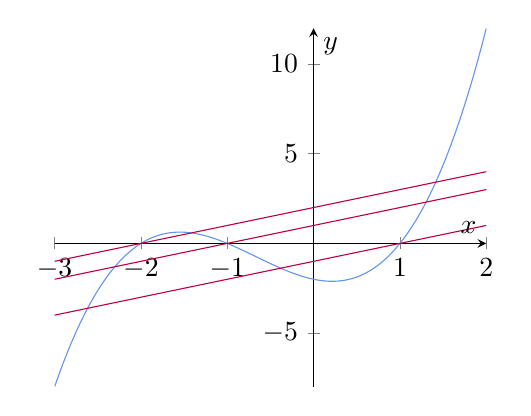
\begin{tikzpicture}
    \begin{axis}[
      xlabel=$x$,
      ylabel={$y$},
      axis lines=middle,
      scale=.8
    ]
      \addplot[domain=-3:2, samples=100, color=CornflowerBlue]{ x^3 + 2*x^2 - x - 2};
      \addplot[domain=-3:2, samples=5, color=purple]{ x - 1 };
      \addplot[domain=-3:2, samples=5, color=purple]{ x + 1 };
      \addplot[domain=-3:2, samples=5, color=purple]{ x + 2 };
    \end{axis}
  \end{tikzpicture}
  \caption{The solutions to an equation are exactly the solutions of its factors.\label{fig:factgraph}}
\end{figure}

If we know that the solutions to a polynomial are integers, we need only try the factors
of the constant term as this term is simply the product of the roots of the polynomial.

One algorithm to divide one polynomial by another is long division, such as the following
calculation which provides us with an example of the division of a polynomial by another that is not a factor.

\begin{center}
  \polylongdiv{x^4 + x - 3}{x^2 - 1}
\end{center}

Here, we have divided $ p(x) = x^4 + x - 3 $ by $ g(x) = x^2 - 1 $ to obtain the quotient $ q(x) = x^2 + 1 $
and the remainder $ r(x) = x - 2 $ --- i.e. we can write $ x^4 + x - 3 = (x^2 - 1)(x^2 + 1) + x - 2 $.

\subsection*{The Remainder Theorem}
One important theorem that follows from the idea of polynomial division is the remainder theorem.

\begin{thm}[Remainder Theorem]
  If we can write $ p(x) = (x-a) q(x) + r $, then $ p(a) = r $.
\end{thm}

Here we are dividing a polynomial $ p(x) $ by some other
linear equation $ (x-a) $, to get a quotient $ q(x) $ and a remainder $ r $
(which is just a number, not a polynomial, in this case). It follows that the
remainder is just the value of $ p(x) $ evaluated at $ a $.

\begin{proof}
  If we substitute $ a $ into the statement above, it simplifies and we obtain that
  $ p(a) = (a - a)q(a) + r = 0\cdot q(a) + r = r $.
\end{proof}

An important consequence of this theorem is that if $ a $ is a solution to the
polynomial, then $ r = p(a) = 0 $ and so $ (x - a) $ is a factor. As we expect,
the solutions to an equation are the same as the solutions to the factors of the equation.

If we can divide out a polynomial multiple times by a factor, we call the
root(s) corresponding to that factor "repeated." The \textit{multiplicity}
of some root $ \alpha $ of $ p(x) = 0 $ is the number of times that the factor
$ (x - \alpha) $ appears in $ p(x) $: i.e. the highest number $ n $ such that the division
of $ p(x) $ by $ (x - \alpha)^n $ gives a remainder of zero. The multiplicity, in some
sense, quantifies the number of times that a root is repeated.

A second application of the remainder theorem is less obvious --- we can
use it to evaluate polynomials. For example, we can use the remainder theorem
to find $ f(4) $ if $ f(x) = 4x^{17} - 4x^{16} + 3x^4 - 6x + 12 $ by dividing $ f(x) $
by $ (x - 4) $ and taking the remainder.

\subsection*{Exercises}
\begin{enumerate}
  \item Find three different polynomials with variable $ x $ that have the two roots $ x = 2 $ and $ x = 3 $.
  \item Show that $ x^6 + x^5 + x^4 + x^3 + x^2 + x + 1 $ divided by $ x^3 + 7 $ gives
        a quotient of $ x^3 + x^2 + x - 6 $ and a remainder of $ -6x^2 - 6x - 41 $ by
        expanding and simplifying $ (x^3 + 7)(x^3 + x^2 + x - 6) + (-6x^2 - 6x - 41) $.
  \item Divide, finding the quotient and remainder polynomials:
        \begin{enumerate*}
          \item $ x^2 - 4 $ by $ x - 2 $,
          \item $ x^2 - 4 $ by $ x - 3 $, and
          \item $ t^7 - t^3 + 5 $ by $ t^3 + 7 $.
        \end{enumerate*}
  \item If $ x = 3 $ is one zero of $ x^3 - 3x^2 - 4x + 12 $, find the other two.
  \item Solve $ x^3 - x^2 - 3x + 3 = 0 $.
  \item Find the roots of $ x^4 - x^3 - 43x^2 + 85x - 42 $.
  \item How many distinct solutions does
        \begin{displaymath}
          (x^2 - 2x - 24)(x^2 + 5x) = (x^2 - 2x - 24)(4x + 12)
        \end{displaymath}
        have?
  \item Show that $ t = 4 $ is a zero of $ t^4 - (6 + \sqrt{3})t^3 + 6\sqrt{3}t^2 + 32t -32\sqrt{3} $.
  \item Find the remainder after dividing $ x^7 + 5x - 9 $ by $ (x-6) $.
  \item Find four polynomials $ p_a(x) $, $ p_b(x) $, $ p_c(x) $, $ p_d(x) $ with integer coefficients such that:
    \begin{enumerate*}
      \item $ p_a\left(\frac{1}{2}\right) = 0 $;
      \item $ p_b\left(\frac{1}{2} + \frac{1}{2} \sqrt{3}\right) = 0 $;
      \item $ p_c\left(2i - \sqrt{2} \right) = 0 $; and
      \item $ p_d\left(\sqrt{i} + \frac{1}{\sqrt[3]{2}}\right) = 0 $.
    \end{enumerate*}
  \hard If $ x^2 + bx + c $ and $ x^2 + dx + e $ have a common factor of $ (x - p) $,
        show that $ \frac{e-c}{b-d} = p $.
  \item Let $ p(x) = (x^2 - 25)^5 $. One root of $ p(x) $ is $ x = 5 $. What is the
        multiplicity of this root?
  \item Is $ (x+3) $ a factor of $ 2x^3 + x^2 - 5x + 7 $?
  \item Use the remainder theorem to compute $ f(3) $ for $ f(x) = x^4 + x - 10 $.
  \item Show that if $ \alpha \neq 0 $ and $ \beta $ are roots of $ x^n - x = 0 $ (for $ n > 1 $), then $ \alpha^{-1} $ and $ \alpha\beta $
        are also roots. Why does this not imply that $ x^2 - x = 0 $ and $ x^3 - x = 0 $ have at least four roots?
  \hard Elliptic curves are a form of cubic; they are equations of the form $ y^2 = x^3 + ax + b $.
        \begin{enumerate}
          \item Find the $ x$-intercepts of $ y^2 = x^3 - 2x $.
          \item Find the $ z$-intercepts of $ y^2 = x^3 - \frac{4}{3} x - \frac{16}{27} $,
                given that $ z = x - \frac{1}{3} $.
          \item Consider an elliptic curve $ \mathcal{E} $, and let $ P $ and $ Q $ be two rational points (i.e. points whose coordinates
                are rational) which are lying on the curve. Let $ \mathcal{L} $ be the chord line uniquely determined by $ P $ and $ Q $. Show
                that if $ \mathcal{L} $ and $ \mathcal{E} $ intersect at a third point $ R $, then this third point is rational.
        \end{enumerate}
  \harder The polynomial $ x^3 + px - 1 $ has three real non-zero roots, $ \alpha $,
        $ \beta $, and~$ \gamma $.
        \begin{enumerate}
          \item Find the value of $ \alpha^2 + \beta^2 + \gamma^2 $ in terms of $ p $,
                and hence show that $ p $ is negative.
          \item Find the cubic polynomial with coefficients in terms of $ p $ with the
                roots $ \alpha^2 $, $ \beta^2 $, and~$ \gamma^2 $.
        \end{enumerate}
  \item Take the general cubic, $ at^3 + bt^2 + ct + d $. Show that the substitution $ t = y - \frac{b}{3a} $
        will give a cubic in $ y $ with no quadratic term (this is known as a Tschirnhaus substitution and is
        often the first step to create a general formula to solve the cubic).
  \item Show that $ \sqrt{2} + \sqrt{3} = \sqrt{5 + \sqrt{6}} $.
  \harder Prove the following identity.\footnote{~See chapter 1 of \cite{Ste15} for historical context.}
        \begin{displaymath}
          \sqrt[3]{-18 + \sqrt{325}} + \sqrt[3]{-18 - \sqrt{325}} = -3
        \end{displaymath}
  \item Let $ w = a + b\sqrt{2} + c\sqrt{3} + d\sqrt{6} $, where $ a $, $ b $, $ c $, and $ d $ are rational.
        Find rational numbers $ p $, $ q $, $ r $ and $ s $ such that
        \begin{displaymath}
          w = p + q(\sqrt{2}  + \sqrt{3}) + r(\sqrt{2} + \sqrt{3})^2 + s(\sqrt{2} + \sqrt{3})^3.
        \end{displaymath}
  \item Show that there are no integers $ r $ and $ s $ such that $ \sqrt{2} = \frac{r}{s} \sqrt{3} $.
\end{enumerate}

\section{Complex Numbers}\label{sec:complex1}
\begin{aquote}{Philip Davis and Reuben Hersh}
  [Mathematics consists of] true facts about imaginary objects.
\end{aquote}
Now that we have somewhat developed the theory of polynomial equations, a sensible question to ask ourselves is the following.
\begin{center}
  \emph{When do polynomial equations have solutions?}
\end{center}
The answer to this simple question is actually quite nuanced, and occupied mathematicians in Europe for centuries.

Consider, for example, the simple quadratic equation
\begin{displaymath}
  x^2 - 2 = 0.
\end{displaymath}
Notice that the coefficients of this equation are integers, but the solutions are not --- in fact, the solutions ($ \pm \sqrt{2} $)
are not even rational! Notice also that the number of solutions is 2, the same as the degree of the polynomial.

Let us take a look at another example,
\begin{displaymath}
  x^3 - x = 0.
\end{displaymath}
Again, the degree of this polynomial is three --- as is the number of solutions that we obtain from it.

These two examples, as well as our previous work, suggest that the number of solutions of a polynomial is the same as its degree. There
is one problem with this, illustrated by another simple equation:
\begin{displaymath}
  x^2 + 1 = 0.
\end{displaymath}

If we try to solve this equation, we end up with a seemingly nonsense result: that $ x = \pm \sqrt{-1} $. Since there is no real
number with a negative square, it seems like we need to throw out our pretty result. However, remember that we have already seen
an example of an equation where the solution is out of reach if we only look for solutions that are the `same kind' as the coefficients.

Just as we extend the natural numbers to the integers, the integers to the rationals, and the rationals to the reals, we can
extend our number system further so that the equation $ x^2 + 1 = 0 $ has a solution. We begin by defining $ i $ to be a square
root of $ -1 $ (and setting $ -i $ to be the other square root); then the set of all numbers of the form $ a + bi $ (for any real
numbers $ a $ and $ b $) is called the set of \emph{complex numbers}; this system of writing them is called \emph{rectangular form}.

The complex numbers are generally considered to have been first used in Girolamo Cardano's \emph{Ars Magna} in 1545, where he
introduces them only to dismiss them as `as subtle as they are useless'. Despite this, modern mathematics has fully accepted the
existence of complex numbers for two main reasons: firstly they do not introduce any contradictions into basic arithmetic or
any theory that we care about, and secondly they allow us to state the following historic theorem.

\begin{thm}[Fundamental Theorem of Algebra]
  Let $ p(x) $ be a polynomial with complex coefficients. Then, counting repeated roots, there are exactly $ \partial p $ complex roots of $ p(x) $.
\end{thm}

The proof of the Fundamental Theorem unfortunately requires concepts and techniques far beyond the scope of this book. All proofs (that I am aware of) require
the use of analysis (i.e. there is no pure-algebra proof).\footnote{~Stewart gives a proof in \cite{Ste15}, and Artin gives two(!) proofs in \cite{Art91} \S 9.9.}

The first rigorous proof of the theorem was published by French mathematician Jean-Robert Argand in 1814; the name is somewhat
incorrect in the modern era as the study of algebra is no longer purely devoted to the properties of the complex number field.
An analogue of the theorem in a more modern context is Kronecker's Theorem, which states that a polynomial with coefficients
in set of numbers in which we can add, subtract, multiply, and divide has at least one solution in a `bigger' set of numbers that
contains the original set.

Given a complex number $ z = a + bi $, we call $ a $ the \emph{real part} of $ z $ and $ b $ the \emph{imaginary part}
of $ z $ (writing $ \realp{z} $ and $ \imagp{z} $ respectively). The term `imaginary' is purely historical --- the complex numbers
exist in exactly the same way that a number like $ \pi = 3.14159... $ or $ e = 2.718... $ exists.

We say that two complex numbers are equal \textbf{if and only if both the real and imaginary parts of those numbers are equal}, and
we perform arithmetic on complex numbers in the same way that we perform arithmetic on the reals, remembering that $ i^2 = -1 $.

Complex numbers also have a geometric interpretation. If we set up a mapping $ a + bi \mapsto (a, b) $ it is easy to see that we
have an exact correspondence between complex numbers and points on a Cartesian plane. This kind of diagram is called an \emph{Argand
diagram}, named after French mathematician Jean-Robert Argand.

For convenience, we also often associate with each complex number the unique \emph{vector} pointing from the origin to the location
of the point on the Argand plane. Given a complex number $ z = a + bi $, the length of its associated vector is called its \emph{modulus};
this is written $ \abs{z} $, and (by the Pythagorean theorem) we have the simple result that $ \abs{z} = \sqrt{a^2 + b^2} $. The meaning
of this is exactly the same as that of the absolute value of a real number (and in fact the modulus of a real number is exactly its absolute
value) --- despite this, note that while there is a natural ordering on the real numbers (for example, $ -2 < 0 < \pi < \sqrt{17} $) there
can be no such ordering on the complex numbers. It is completely nonsensical to talk about any complex number being `bigger' than any other.

\begin{figure}
  \centering
  \begin{tikzpicture}
    \begin{axis}[
      xmin = -4, xmax = 4,
      ymin = -4, ymax = 4,
      xlabel=$\realp{z}$,
      ylabel={$\imagp{z}$},
      axis lines=middle,
      scale=.8
    ]
      \addplot[color=BurntOrange, mark=*, thick]
      coordinates {
        (0, 1)
      };
      \addplot[color=ForestGreen, mark=*, thick]
      coordinates {
        (1, 0)
      };
      \addplot[color=NavyBlue, mark=*, thick]
      coordinates {
        (3,2)
      };
      \addplot[color=Red, mark=*, thick]
      coordinates {
        (-1,-1)
      };
      \addplot[color=Mulberry, mark=*, thick]
      coordinates {
        (-1,2)
      };
    \end{axis}
  \end{tikzpicture}
  \caption{Five points on an Argand diagram.\label{fig:argand}}
\end{figure}

The five points marked on the Argand diagram in \cref{fig:argand} are $ i $, 1, $ 3+2i $, $ -1 - i $, and $ 2i - 1 $. See if you
can label each point on the diagram itself.

\subsection*{Addition and Subtraction}
Due to the way we constructed the complex numbers, there are natural rules for arithmetic. Suppose we have two complex numbers, $ u = a + bi $
and $ v = c + di $. We have the following rules for addition and subtraction by collecting the real and imaginary terms together:
\begin{align*}
  u + v &= (a + c) + (b + d)i, \text{ and} \\
  u - v &= (a - c) + (b - d)i.
\end{align*}

Geometrically, we are simply taking the vectors associated with each point and adding them.

\begin{figure}
  \centering
  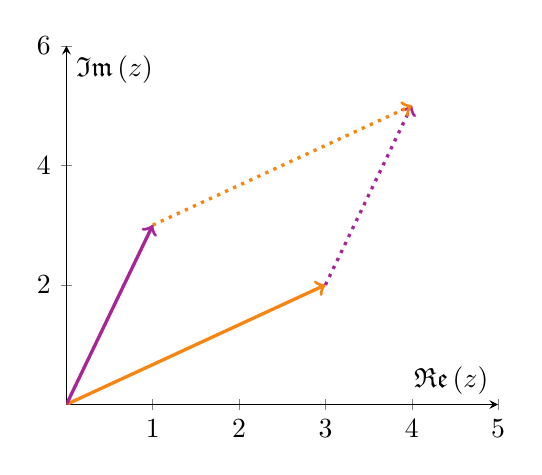
\begin{tikzpicture}
    \begin{axis}[
      xmin = 0, xmax = 5,
      ymin = 0, ymax = 6,
      xlabel=$\realp{z}$,
      ylabel={$\imagp{z}$},
      axis lines=middle,
      scale=.8
    ]
      \coordinate (O) at (0,0);
      \coordinate (A) at (3,2);
      \coordinate (B) at (1,3);
      \coordinate (S) at (4,5);
      \draw[very thick, BurntOrange, ->] (O)--(A);
      \draw[very thick, dotted, Mulberry, ->] (A)--(S);
      \draw[very thick, dotted, BurntOrange, ->] (B)--(S);
      \draw[very thick, Mulberry, ->] (O)--(B);
    \end{axis}
  \end{tikzpicture}
  \caption{The addition of complex numbers.}
\end{figure}

Before we discuss multiplication of complex numbers, we will discuss one more simple but important operation: that of complex conjugation. Our intent
is to take the geometric property of reflection (across the real axis), and give it an algebraic meaning; in particular, the \emph{complex conjugate}
of $ z = a + bi $ is $ \overline z = a-bi $. An initial application of this concept is the simple result that if a polynomial has real coefficents,
any complex roots must come in conjugate pairs (you are asked to prove this in the special case of quadratic polynomials as exercise \ref{ex:conjquadratic},
and in the general case as exercise \ref{sec:finalexs}.\ref{ex:solutiongenerator}).

\subsection*{Multiplication}
There is a rule for multiplying complex numbers that is similar to the rules for addition; we simply collect like
terms and remember that $ i^2 = -1 $ in order to obtain the result
\begin{displaymath}
  (a+bi)(c+di) = ac + adi + bci + bdi^2 = (ac - bd) + (ad + bc)i.
\end{displaymath}

This way of writing the result is a little esoteric and has no nice geometric meaning. In order to remedy this problem, we rewrite our
complex numbers in \emph{polar form}. Instead of writing the number in the form $ z = a + bi $, where $ a $ and $ b $
are the distances from the two axes, we write $ z = r \cis \theta $, where $ r $ is the distance of the number from the
origin (simply the modulus $ \abs{z} $ again) and $ \theta $ is the angle that number's vector makes with the $ x$-axis
(known as the \emph{argument} of $ z $, and written as $ \carg(z) $). The function $ \cis \theta $ is defined to be $ \cos \theta + i\sin \theta $.

\begin{figure}
  \centering
  \begin{tikzpicture}
    \begin{axis}[
      xmin = 0, xmax = 4,
      ymin = 0, ymax = 3,
      xticklabels = {,,},
      yticklabels = {,,},
      ticks=none,
      xlabel=$\realp{z}$,
      ylabel={$\imagp{z}$},
      axis lines=middle
    ]
      \coordinate (O) at (0,0);
      \node[circle, fill=ForestGreen, inner sep=0pt, minimum size=5pt, label=above right:{$ z = a + bi $}] (A) at (3,2) {};
      \coordinate (B) at (3,0);
      \draw[black, ->] (O)--(A) node[midway, sloped, above left] {$ r $};
      \draw[black] (O) +(0:.8cm) arc (0:33.69:.9cm);
      \draw[black] (O) +(15:.6) node[rotate=0] {$ \theta $};
      \draw[black] (B) -- (A) node[midway, right] {$ b $};
      \draw[black] (O) -- (B) node[midway, above] {$ a $};
    \end{axis}
  \end{tikzpicture}
  \caption{The polar form of a complex number.}
\end{figure}

It is simple to see that $ \theta = \tan^{-1}{\frac{b}{a}} $; we have already got a formula for $ r $.

This new notation simplifies multiplication significantly, because you will show as an exercise that
\begin{displaymath}
  (r \cis \theta)(t \cis \varphi) = (rt) \cis (\theta + \varphi).
\end{displaymath}

For example, if we were to multiply $ 3 \cis \pi $ by $ 4 \cis \pi $, we would obtain $ 12 \cis 2\pi = 12 $. This is as expected,
as $ p \cis \pi = -p $, and $ -3 \times -4 = 12 $.

Note that any complex number has an infinite number of different representations in polar form, simply by adding $ 2\pi $ (an entire
rotation around the origin) to its argument. This fact comes into play later on when we try to solve equations involving powers of complex
numbers.

\subsection*{Exponentiation}
Finally, we ask ourselves what a definition of complex exponentiation should be. There are two important
behaviours of the real exponential function which we want to preserve: the sum-to-product rule ($ \exp(x + y) = \exp(x) \exp(y) $)
and the differentiation rule ($ \exp'(x) = \exp(x) $).

If we define the complex exponential in such a way that these rules hold, then we will have $ \exp(x + iy) = \exp(x) \exp(iy) $;
in particular, we need only make a sensible definition for $ \exp(iy) $. Further, we have already seen a function that satisfies the sum
rule: $ \cis(x + y) = \cis(x) \cis(y) $. Thus, we make a guess that a decent definition for our exponential function will be $ \exp(iy) = \cis(y) $.

We now check that this definition satisfies the differentiation rule: we have not formally defined how differentiation should work over the
complex numbers, but $ \cis $ is only a function of real variables and so we can differentiate it using our normal definitions:
\begin{displaymath}
  \od{}{y} [\cos y + i\sin y] = -\sin y + i\cos y = i(i\sin y + \cos y) = i\cis y.
\end{displaymath}
Thus, if we make this definition, then $ \exp(iy) = i\exp(iy) $ which is the `usual' rule for exponent differentiation.

We therefore make the definition formally, known as \emph{Euler's formula}, that
\begin{displaymath}
  \cis \theta = \exp(i\theta)
\end{displaymath}
and thus
\begin{displaymath}
  \exp(x + iy) = e^x \cis y;
\end{displaymath}
we will also allow ourselves to use the standard notation, $ \exp(z) = e^z $.

Philosophically, we make the note that complex exponentiation is very elegant, in the sense that it
is simply a function which transforms numbers from rectangular form into polar form by `wrapping them
around the origin'!

From Euler's formula we obtain the following equation, which relates five fundamental mathematical constants
in one expression and which some have called the most beautiful equation in mathematics:
\begin{equation}
  \tag{Euler's Identity}
  e^{i\pi} + 1 = 0.
\end{equation}

\begin{figure}
  \centering
  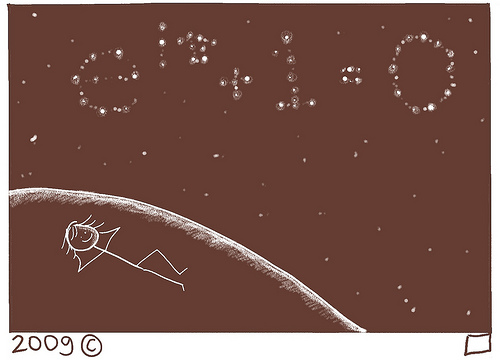
\includegraphics[width=0.4\textwidth]{stars}
  \caption{From \url{http://brownsharpie.courtneygibbons.org/?p=848}.}
\end{figure}

\subsection*{Exercises}
\begin{enumerate}
  \item Evaluate the following expressions, and plot the answers on an Argand diagram:
        \begin{enumerate}
          \item $ (3+2i) + (6-2i) $
          \item $ 24 - (6 + 2i) $
          \item $ 2(2+i) + 6i - 7 $
        \end{enumerate}
  \item If we add two real numbers, can we obtain an imaginary number? If we add two
        imaginary numbers, can we obtain a real number?
  \item Let $ v = 3-7i $ and $ w = -4+6i $.
    \begin{enumerate}
      \item Find the real numbers $ p $ and $ q $ such that $ pv + qw = 6.5 - 11i $.
      \item Show that any complex number $ z $ can be written as $ z = pv + qw $ for some real $ p $ and $ q $.
    \end{enumerate}
  \item Solve the quadratic equation $ x^2 + 4 = 0 $.
  \item Prove that $ z + \overline z = 2 \cdot \realp{z} $ and $ z - \overline z = 2i \cdot \imagp{z} $. \label{ex:reflecsum}
  \item Verify the following properties of conjugation.
    \begin{enumerate}
      \item $ \overline {\overline z} = z $
      \item $ \overline w + \overline z = \overline{w + z} $
      \item $ \overline w \overline z = \overline{wz} $
    \end{enumerate}
  \item Find $ i^{957} $.
  \item Show that $ \abs{a + bi} \geq \abs{a} $ and $ \abs{a + bi} \geq \abs{b} $.
  \item Find $ (3 + 2i)(6 + 8i) $ in rectangular form.
  \item \begin{enumerate}
          \item Convert $ 1 + i $ into polar form.
          \item Find $ (1 + i)(\sqrt{2} \cis \frac{3\pi}{4}) $ in both polar form and rectangular form.
        \end{enumerate}
  \item Compute $ (6 \cis \frac{23\pi}{24})(9\cis \frac{14\pi}{17}) $, leaving your answer in polar form.
  \item \begin{enumerate}
          \item Prove that $ (r \cis \theta)(t \cis \varphi) = (rt) \cis (\theta + \varphi) $.
          \item Describe the geometric meaning of the multiplication of complex numbers.
        \end{enumerate}
  \item Let $ u = 2 \cis \frac{\pi}{2} $ and $ v = 3 \cis \frac{3\pi}{2} $. Plot $ u $, $ v $, and $ uv $ on an Argand diagram.
  \item Prove \textbf{de Moivre's Theorem}: $ (r \cis \theta)^n = (r^n) \cis (n\theta) $.
  \item Show that if $ u = r \cis \theta $ and $ v = t \cis \varphi $ then $ \frac{u}{v} = \frac{r}{t}\cis(\theta - \varphi) $.
  \item Using de Moirve's Theorem, prove that for complex numbers $ w $ and $ m $ and integers $ n $ and $ m $,
    \begin{enumerate*}
      \item $ w^n w^m = w^{n + m} $, and
      \item $ (w^n)^m = w^{nm} $.
    \end{enumerate*}
  \item Convert $ w = 1 + \sqrt{3}i $ into polar form, and calculate $ w^3 $.
  \item Show that for any complex number $ z $, the product $ z \overline z $ is both real and non-negative.
        Hence show that $ (x - z)(x - \overline z) $ has only real coeffients.
  \item Let $ x $ be a real number. Show that, for all integers $ n $, $ \cis \frac{2x\pi}{n} = \cis \frac{2(x + n)\pi}{n} $.
  \item For which complex numbers is $ z^2 $ real? What about $ z^3 $?
  \item Transform $ \frac{a+bi}{c+di} $ so that the only imaginary part is in the numerator.
  \item Find $ (a+bi)^{-1} $ in rectangular form.
  \item Write the complex number $ \left( \frac{4i^7 - i}{1+2i} \right)^2 $ in the
        form $ a + bi $, where $ a $ and $ b $ are real numbers.
  \item
    \begin{enumerate}
      \item Prove that a number $ z $ is real if and only if $ \overline z = z $.
      \item Hence, or otherwise, show that $ z \overline w + w \overline z $ is always real.
      \item Show that $ z \overline w + w \overline z \leq 2 \abs{w} \abs{z} $.
    \end{enumerate}
  \item Show that if $ z = a + ib $ then $ \sqrt{z\overline z} = \abs{z} $.
  \hard If $ \zeta = \sqrt{\frac{1}{2}(a+\sqrt{a^2+b^2})} + i\sqrt{\frac{1}{2}(-a+\sqrt{a^2+b^2})} $
        is a complex number, find $ \zeta^2 $ in the form $ p + iq $ (where $ a $, $ b $, $ p $, and $ q $ are real).
  \hard If $ z = x + iy $, and $ az^2 + bz + c = 0 $, show that $ a \overline z^2 + b \overline z + c = 0 $
        if $ a $, $ b $, and $ c $ are real. (This exercise is generalised in \ref{sec:finalexs}.\ref{ex:solutiongenerator}.) \label{ex:conjquadratic}
  \hard Use Euler's identity to find $ \ln (-1) $, and hence $ \ln (-x) $ for real $ x $.
  \hard Prove that for every positive integer $ n $, $ (-1 + \sqrt{3}i)^{3n} + (-1 - \sqrt{3}i)^{3n} = 2^{3n+1} $.
  \item Show that $ y_1(x) = e^{ix} + e^{-ix} $ and $ y_2(x) = 2\cos x $ are both solutions of the differential equation
        \begin{displaymath}
          \od[2]{y}{x} + y = 0
        \end{displaymath}
        with initial conditions $ y(0) = 2 $ and $ y'(0) = 0 $. (Also see \ref{ex:eulersin} below.)
  \item Find $ \sqrt{i} $ in rectangular form.
  \item\label{ex:eulersin}
    \begin{enumerate}
      \item Show that $ \cos \theta = \frac{e^{i\theta} + e^{-i\theta}}{2} $ and that $ \sin \theta = \frac{e^{i\theta} - e^{-i\theta}}{2i} $.
      \item If $ x + x^{-1} = 2 \cos \theta $, find $ x^n + x^{-n} $ in terms of $ n $ and $ \theta $.
    \end{enumerate}
  \item
    \label{ex:cardano}
    \begin{enumerate}
      \item Show that $ (2 \pm i)^3 = 2 \pm 11i $.
      \item Simplify fully $ \sqrt[3]{2+\sqrt{-121}} + \sqrt[3]{2-\sqrt{-121}} $.
      \item Show that (b) is a root of the cubic equation $ t^3 - 15t - 4 = 0 $,
            and hence find all three solutions.
    \end{enumerate}
  \item You do not need the fundamental theorem of algebra for this exercise.
    \begin{enumerate}
      \item Prove that all cubic equations with real coefficients must have exactly three roots in the complex numbers.
      \item Let $ p(x) $ be a polynomial of degree $ n $ such that there exists some complex number $ \zeta $ such that $ p(\zeta) = 0 $.
            Show that $ p(x) = 0 $ has exactly $ n $ solutions (counting repeated roots).
    \end{enumerate}
\end{enumerate}

\section{Geometry}\label{sec:geometry}
\begin{aquote}{Michael Atiyah}
  Algebra is the offer made by the devil to the mathematician... All you need to do, is give me your soul: give up geometry.
\end{aquote}
We have already seen that we can view the complex numbers as points in the plane, $ \mathbb{R}^2 $. This means
that we can carry out geometric operations algebraically using complex numbers. For example, the length of the line joining two
points $ z_1 $ and $ z_2 $ is simply $ \abs{z_1 - z_2} $.

We define the \textit{locus} of an equation to be the set of all points satisfying that equation; for example, the locus
of $ x^2 + y^2 = 1 $ is the set of all points making up the unit circle. We can use our correspondence between points on
a plane and complex numbers to reason about the locus of a complex equation; for example, the locus of the equation $ \abs{z} = 1 $
is the set of all points at a unit distance from the origin: it is another way of talking about the unit circle. (If you
write $ z = x + iy $, then $ \abs{z} = x^2 + y^2 $ and the comparison becomes even more obvious.)

More interestingly, consider the set of all points $ z $ such that for some real number $ t $ and for a pair of fixed
points $ z_1 $ and $ z_2 $, $ z = tz_1 + (1 - t)z_2 $. The locus of this set is the line joining $ z_1 $ and $ z_2 $.
To prove this, write $ z = x + iy $, $ z_1 = x_1 + iy_1 $, and $ z_2 = x_2 + iy_2 $; then the equation tells us that
\begin{gather*}
  x + yi = tx_1 + it y_1 + x_2 + i y_2 - tx_2 - it y_2\\
  x = t(x_1 - x_2) + x_2, \qquad y = t(y_1 - y_2) + y_2
\end{gather*}
From the second line, we see that $ t = \frac{x - x_2}{x_1 - x_2} $ and thus
\begin{gather*}
  y = \frac{x - x_2}{x_1 - x_2}(y_1 - y_2) + y_2.
\end{gather*}
Writing $ m = \frac{y_1 - y_2}{x_1 - x_2} $, we see that we have the equation of a line passing through $ (x_2, y_2) $
with slope $ m $.

Now, we will consider two non-zero complex numbers $ w $ and $ z $; we will call the two points \textit{orthogonal} if the lines
passing from $ w $ and $ z $ to the origin meet at right angles. The claim is that the two points are orthogonal precisely
when $ \realp w \realp z + \imagp w \imagp z = 0 $. Suppose that the two points are orthogonal; then, by Pythagoras' theorem,
we have that $ \abs{w - z}^2 = \abs{w}^2 + \abs{z}^2 $. Expanding this, we obtain
\begin{align*}
  (w - z)(\overline{w} - \overline{z}) &= w\overline{w} + z\overline{z}\\
  z\overline{w} + w\overline{z} &= 0.
\end{align*}
But $ z\overline{w} + w\overline{z} = z \overline{w} + \overline{z \overline{w}} $, and hence (applying exercise \ref{sec:complex1}.\ref{ex:reflecsum})
we have $ 2 \realp{z \overline{w}} = 0 $. But $ \realp{z \overline w} = \realp{z}\realp{w} + \imagp{z} \imagp{w} $, and so the condition
claimed holds.

On the other hand, suppose $ \realp{z}\realp{w} + \imagp{z} \imagp{w} = 0 $. We form the triangle with sides $ \abs{w} $, $ \abs{z} $,
and $ \abs{w - z} $ with an angle $ \theta $ at the origin. By the cosine rule, $ \abs{w - z}^2 = \abs{w}^2 + \abs{z}^2 - 2\abs{w}\abs{z}\cos\theta $.
Using the same argument as above, we have $ z\overline{w} + w\overline{z} = - 2\abs{w}\abs{z}\cos\theta $; but the left hand side
is zero, and thus (since $ \abs{w} $ and $ \abs{z} $ are non-zero) we have $ \cos \theta = 0 $ and $ \theta = \pm \pi/2 $ as claimed.

We call the expression $ \realp w \realp z + \imagp w \imagp z $ the \emph{dot product} of $ w $ and $ z $; we write it $ (w, z) $. One
important property of the dot product is that $ (u + v, w) = (u, w) + (v, w) $.

The dot product is intimately connected with the geometry of the complex plane. As well as our result about orthogonality above,
we have two more properties:
\begin{enumerate}
  \item The modulus of $ z $ is $ \abs{z} = \sqrt{(z, z)} $.
  \item If $ \theta $ is the angle at the origin between $ w $ and $ z $ (i.e. $ \theta = \arg w - \arg z $), then $ \cos \theta = \frac{(w,z)}{\abs{w}\abs{z}} $.
\end{enumerate}

Suppose we have two nonzero complex numbers, $ w_0 $ and $ z_0 $. We want to find the closest point $ z $ on the line generated by $ z_0 $
(i.e. the line passing through $ z_0 $ and the origin) to the point $ w_0 $. This point is called the \emph{projection} of $ w_0 $ onto $ z_0 $,
and we denote it by $ z = \proj_{z_0}(w_0) $.

The calculation of the projection is based on the dot product, and proceeds as follows. Consider $ h = w_0 - tz_0 $, where $ t $ is some
real number. Then $ (h, z_0) = (w_0, z_0) - (tz_0, z_0) = (w_0, z_0) - t\abs{z_0}^2 $; so $ h $ is perpendicular to $ tz_0 $ precisely
when $ t = \frac{(w_0, z_0)}{\abs{z_0}^2} = \frac{(w_0, z_0)}{(z_0, z_0)} $. It follows that
\begin{displaymath}
  \proj_{z_0}(w_0) = z_0 \frac{(w_0, z_0)}{(z_0, z_0)}.
\end{displaymath}
This result tells us that the geometric meaning of the dot product $ (a,b) $ is just the length of the `shadow' cast onto $ a $
by $ b $, multiplied by the squared length of $ a $. But the dot product is symmetric, so this is also the length of the `shadow' cast onto $ b $
by $ a $, multiplied by the squared length of $ b $. If both $ a $ and $ b $ have length 1, then this length is just the cosine of
the angle between them. (See \cref{fig:projection}.)

\begin{figure}
  \centering
  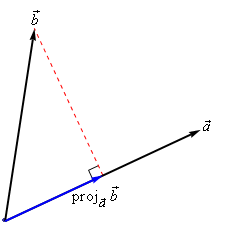
\includegraphics[width=0.2\textwidth]{projection}
  \caption{The projection of $ b $ onto $ a $. From \url{http://tutorial.math.lamar.edu/Classes/CalcII/DotProduct.aspx}.\label{fig:projection}}
\end{figure}

As a bonus, if we are given any fixed complex number $ z_0 $ then we can write every vector $ w_0 $ in the plane in the form $ w_0 = tz_0 + z_0^\perp $
where $ z_0 $ and $ z_0^\perp $ are perpendicular: just take $ t = \frac{(w_0, z_0)}{(z_0, z_0)} $ and $ z_0^\perp = w_0 - tz_0 $.

Another important geometric property of the complex numbers is the triangle inequality; if $ a $ and $ b $ are
complex numbers, then $ \abs{a + b} \leq \abs{a} + \abs{b} $. Geometrically, this just states that if two sides
of a triangle have lengths $ \abs{a} $ and $ \abs{b} $ then the third side has length at most $ \abs{a} + \abs{b} $ (\cref{fig:triangleineq}).

\begin{figure}
  \centering
  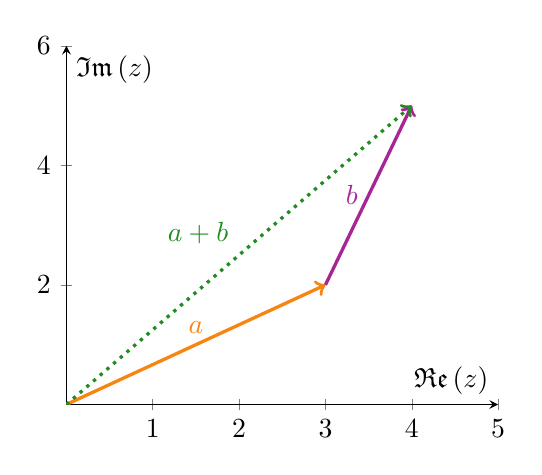
\begin{tikzpicture}
    \begin{axis}[
      xmin = 0, xmax = 5,
      ymin = 0, ymax = 6,
      xlabel=$\realp{z}$,
      ylabel={$\imagp{z}$},
      axis lines=middle,
      scale=.8
    ]
      \coordinate (O) at (0,0);
      \coordinate (A) at (3,2);
      \coordinate (B) at (1,3);
      \coordinate (S) at (4,5);
      \draw[very thick, BurntOrange, ->] (O) -- (A) node[midway,above]{$a$};
      \draw[very thick, Mulberry, ->] (A) -- (S) node[midway,left]{$b$};
      \draw[very thick, dotted, ForestGreen, ->] (O) -- (S) node[midway,above left]{$a+b$};
    \end{axis}
  \end{tikzpicture}
  \caption{The triangle inequality.\label{fig:triangleineq}}
\end{figure}

\subsection*{Exercises}
\begin{enumerate}
  \item Show that, if $ a $ and $ b $ are fixed complex numbers, then $ \abs{z - a} = \abs{z - b} $ describes the line which
        cuts the midpoint of the segment between $ a $ and $ b $ at a right angle.
  \item Let $ v = 1 + i $ and $ z = x + iy $ for any real numbers $ x $ and $ y $.
    \begin{enumerate}
      \item Show that the equation $ \abs{z - v} = \abs{vz} $ represents a circle, and find its
            centre and radius.
      \item Find the point of intersection of the circle with the straight line $ \abs{z - v} = \abs{z + v} $.
    \end{enumerate}
  \item Find the locus of all $ z $ such that for some fixed $ a $, $ z - a $ is perpendicular to $ z + a $.
  \item Show that if $ u $, $ v $, and $ w $ are complex numbers, and if $ \lambda $ and $ \mu $ are real
        numbers, then:
    \begin{enumerate}
      \item $ (u, v) = (v, u) $
      \item $ (\lambda u + \mu v, w) = \lambda(u, w) + \mu(v, w) $
    \end{enumerate}
  \hard Show that if $ b $ is a complex number and $ a $ and $ c $ are real numbers, then the locus of all complex numbers
        $ z $ satisfying $ a(z,z) + (b,z) + c = 0 $ is a circle. (Hint: if $ z $ was real, you would complete the square.)
  \item Let $ X $ be a set of complex numbers. If $ \rho \neq 0 $ and $ t $ are complex numbers, define $ \rho X + t $ to be
        the set of all complex numbers of the form $ \rho x + t $ for some $ x $ in the set $ X $. Show that
      \begin{enumerate*}
        \item if $ X $ is a line, then $ \rho X + t $ is a line;
        \item if $ X $ is a circle, then $ \rho X + t $ is a circle.
      \end{enumerate*}
  \item Let $ p $ be a positive real number, and let $ \Gamma $ be the locus of points $ z $ satisfying $ \abs{z - p} = c\realp{z} $. Show
        that $ \Gamma $ is:
    \begin{enumerate}
      \item an ellipse if $ 0 < c < 1 $;
      \item a parabola if $ c = 1 $;
      \item a hyperbola if $ c > 1 $.
    \end{enumerate}
  \item A set of complex numbers is called \emph{convex} if for every pair of complex numbers in the set the line segment joining
        them is also in the set.
    \begin{enumerate}
      \item Show that the set of all $ z $ where $ \abs{z} < 1 $ is convex.
      \item Show that the set of all $ z $ where $ 0 < \abs{z} < 1 $ is not convex.
    \end{enumerate}
  \item A set of complex numbers is called \emph{star shaped} if there is some point $ c $ in the set such that for every
        other point $ p $ in the set, the segment joining $ p $ to $ c $ lies in the set. Show that every convex set is star shaped.
  \harder If $ S $ is a set of finitely many complex numbers $ z_1, ..., z_n $, the \emph{convex hull} of $ S $ is the smallest convex set
          containing every point of $ S $. Show that a point $ w $ is in the convex hull of $ S $ precisely when there exist $ n $
          non-negative real numbers, $ \lambda_1, ..., \lambda_n $, such that $ \lambda_1 + \cdots + \lambda_n = 1 $, and
          \begin{displaymath}
            w = \lambda_1 z_1 + \cdots \lambda_n z_n.
          \end{displaymath}
          The points $ w $ are called \emph{convex combinations} of the $ z_i $.
  \hard The following inequality, which holds for all real numbers $ a_1 $, $ a_2 $, ..., $ a_n $, $ b_1 $, ..., $ b_n $, is known as the Cauchy-Schwarz
        inequality.
        \begin{equation}\label{eqn:cauchy}
          (a_1 b_1 + a_2 b_2 + \cdots + a_n b_n)^2 \leq (a_1^2 + \cdots + a_n^2)(b_1^2 + \cdots + b_n^2) \tag{Cauchy-Schwarz}
        \end{equation}
        The inequality is a very useful result in analysis; there are several different elementary proofs of it.
        \begin{enumerate}
          \item Show that if $ a > 0 $, then $ ax^2 + bx + c \geq 0 $ for all $ x $ if and only if $ b^2 - 4ac \leq 0 $.
          \item Prove the Cauchy-Schwarz inequality by considering the expression $ (a_1 x + b_1)^2 + \cdots + (a_n x + b_n)^2 $,
                collecting terms, and applying (a).
          \item As a special case of the inequality, show that if $ w $ and $ z $ are complex numbers then $ (w, z)^2 \leq \abs{w}^2 \abs{z}^2 $.
          \item Hence show the \emph{triangle inequality}: $ \abs{a + b} \leq \abs{a} + \abs{b} $ for complex numbers $ a $ and $ b $.
        \end{enumerate}
  \item Multiplication by $ i $ rotates a point by $ \frac{\pi}{2} $ around the origin.
        \begin{enumerate}
          \item A generalisation of this allows us to rotate a point $ z $ around an arbitrary point $ a $ by that
                angle: $ z' = a + i(z-a) $. Justify this formula.
          \item Consider a treasure map with the following instructions:

                \begin{quote}
                  From the statue of Richard Seddon, go to the kauri tree (counting your steps), and then turn
                  exactly 90\degree left and walk the same number of steps to the point $ g' $. Returning
                  to the statue, walk to the beech tree (again counting your steps). Turn right by 90\degree,
                  and walk the same number of steps to point $ g'' $. The treasure is buried exactly at the midpoint
                  of the line joining $ g' $ and $ g'' $.
                \end{quote}

                Given that the kauri tree is at $ (0,0) $, the beech tree is at $ (10,0) $, and
                the statue is somewhere on the line $ y = 2009 $, find the location of the treasure.
          \end{enumerate}
  \hard A line in $ \mathbb{C}^2 $ (the plane with complex coordinates) is defined to be the locus of a linear equation
        $ ax + by + c = 0 $ where $ a $, $ b $, and $ c $ are complex constants. Prove that, given two distinct points $ (x_0, y_0) $
        and $ (x_1, y_1) $ in $ \mathbb{C}^2 $, there is a \textbf{unique} line through those two points. \textit{Hint: it is certainly \textbf{not} true
        that there is a unique linear equation whose graph includes both points.}
  \hard Investigate the locus of $ \left\{z = r\cis\theta : r = \cos\left(\frac{n}{d}\theta\right)\right\} $ for different values of $ n $
        and $ d $.
\end{enumerate}

\section{Roots of Unity}\label{sec:roots}
Let us take the equation $ z^3 = 1 $. We know that this equation has exactly three complex
roots, and of these we already know that the only real root is $ z = 1 $. How can we find
the two non-real roots?

Noting that $ 1 = 1 \cis 2k\pi $ for all natural numbers $ k $, we can apply de~Moivre's~Theorem
to show that $ 1^{(\frac{1}{3})} = \cis \frac{2k\pi}{3} $.

We can then set $ n $ to 0, 1, and 2 to obtain our three roots of the original
equation: $ z = 1 $, $ z = \cis \frac{2\pi}{3} $, and $ z = \cis \frac{4\pi}{3} $
respectively. Note that if we set $ k $ to any higher number (3, for example) we
obtain one of the roots we already have (e.g. $ \cis \frac{6\pi}{3} = 1 $), since we
have gone `around the circle'.

\begin{figure}
  \centering
  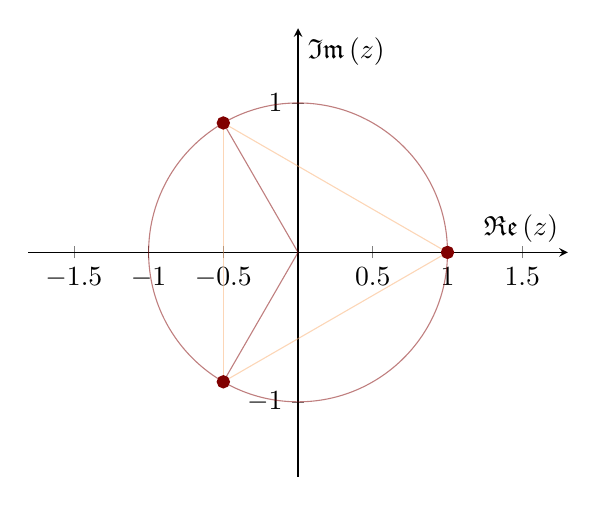
\begin{tikzpicture}
    \begin{axis}[
      xlabel=$\realp{z}$,
      ylabel={$\imagp{z}$},
      axis lines=middle,
      disabledatascaling,
      xmin=-1.5,
      xmax=1.5,
      ymin=-1.5,
      ymax=1.5,
      axis equal
    ]
      \addplot[color=Maroon, mark=*, thick]
      coordinates {
        (1, 0)
      };
      \addplot[color=Maroon, mark=*, thick]
      coordinates {
        (-0.5, 0.866)
      };
      \addplot[color=Maroon, mark=*, thick]
      coordinates {
        (-0.5, -0.866)
      };
    \path [draw=Maroon, fill=none, semitransparent] (0,0) circle (1);
    \path [draw=Maroon, fill=none, semitransparent] (-0.5,0.866) -- (0,0);
    \path [draw=Maroon, fill=none, semitransparent] (-0.5,-0.866) -- (0,0);
    \path [draw=Apricot, fill=none, semitransparent] (-0.5,-0.866) -- (-0.5,0.866);
    \path [draw=Apricot, fill=none, semitransparent] (1, 0) -- (-0.5,0.866);
    \path [draw=Apricot, fill=none, semitransparent] (-0.5,-0.866) -- (1, 0);
    \end{axis}
  \end{tikzpicture}
  \caption{The cube roots of 1.\label{fig:cuberoots}}
\end{figure}

If we look at the roots geometrically (on an Argand diagram like that in \cref{fig:cuberoots}), we see that
the $ n$th roots of 1 will be arranged in a circle of radius $ 1 $ centred on the origin, and the
angles between them will be exactly $ \frac{2\pi}{n} $. If $ n $ is even, both 1 and -1 will both
be real roots, but if $ n $ is odd then 1 will be the only real root. In general, the sum of all
$ n $ $n$th roots of unity is zero (see exercise \ref{ex:rootsum}).

Any integer power of an $n$th root of unity is also an $n$th root of unity. However, not
all $ n$th roots will "generate" all the other ones in this way; for example, $ \cis \frac{2\pi}{3} $
is a sixth root of unity but will miss out every second sixth root if we raise it to integer
powers. Roots which \emph{do} generate all the others are called \emph{primitive roots of unity}.

We formally define a primitive $n$th root of unity to be a complex number $ \omega $ such that $ \omega^n = 1$
but $ \omega^k \neq 1 $ for all $ k < n $. In other words, if we list all the roots of unity in order for $ n = 1,~2,~3 $
and so on, then a root is only primitive for that value of $ n $ for which it first appears.

For example, $ \mu = \cis \frac{2\pi}{3} $ is a primitive third root of unity (since the smallest
nonzero $ n $ such that $ \mu^n = 1 $ is $ n = 3 $).

We now prove that, as we claimed, the primitive $n$th roots of unity "generate" all the other
$ n$th roots of unity:
\begin{thm}
  Given the polynomial $ z^n = 1 $, with primitive root $ \omega $, all solutions
  are given by $ \omega^k $ for $ 0 \leq k \leq (n - 1) $. In other words,
  the integer powers of a primitive $ n$th root of unity must be \emph{all} the
  $n$th roots of unity.
\end{thm}

\begin{proof}
  We first prove that all the powers $ \omega^k $ for $ k $ defined above are distinct.
  Suppose that there are two values for $ k $, say
  $ k = a $ and $ k = b $, such that $ \omega^a = \omega^b $ and $ a \neq b $. Then we have
  that $ \omega^{a-b} = 1 $ and therefore $ a - b = 0 $ (the other possibility here would be
  that $ a - b $ were equal to some non-zero multiple of $ n $, none of which are possible
  values of $ k $) so $ a = b $.

  Since there are $ n $ possible values for $ k $, there are $ n $ distinct powers of $ \omega $
  which are all roots of the polynomial. However, the polynomial is of degree $ n $ and so has
  exactly $ n $ roots --- thus, the powers of $ \omega $ are exactly the roots of the polynomial.
\end{proof}

Roots of unity allow us to find all the $ n$th roots of any number easily. Suppose $ a^n = x $; then
the $ n$th roots of $ x $ will be $ a = \omega^k \sqrt[n]{x} $ ($ 0 \leq k < n $) where $ \omega $ is a
primitive $ n$th root of unity and $ \sqrt[n]{x} $ is any $ n$th root of $ x $.

\subsection*{Exercises}
For the exercises marked $ \dagger $, it may be useful to use the result that for all integers $ a $ and $ b $
there exist integers $ m $ and $ n $ such that $ am + bn = \gcd(a,b) $ (where the $ \gcd $ of two numbers is the
largest integer that divides into both of them). Two integers $ a $ and $ b $ are coprime if they share
no divisors (i.e. if $ \gcd(a,b) = 1 $).
\begin{enumerate}
  \item Let $ p(z) = z^5 - 1 $.
    \begin{enumerate}
      \item Find exactly each of the roots of $ p(z) $.
      \item Let $ \alpha $ be the root of $ p $ with the smallest non-zero
            positive argument. Show explicitly that the roots can be written as 1, $ \alpha $,
            $ \alpha^2 $, $ \alpha^3 $, and $ \alpha^4 $.
    \end{enumerate}
  \item Find all solutions of $ z^3 + n = 0 $, where $ n $ is a positive real number,
        in exact form in terms of $ n $.
  \item Solve for $ z $ if $ (z-3)^7 = 1 $.
  \item Find the fifth roots of $ 4 + 4i $ in polar form, and draw them on an Argand
        diagram. Hence find integers $ p $ and $ q $ such that $ (p+qi)^5 = (4+4i) $.
  \item Write down all of the primitive sixth roots of unity. What about the primitive fifth roots of unity?
  \hard \label{ex:rootsum}
    \begin{enumerate}
      \item Let $ \alpha $ be a complex root of $ x^3 = 1 $. Show by computation that $ \alpha^2 + \alpha + 1 = 0 $.
      \item In general, prove that the sum of all $ n $ $ n$th roots of unity is zero (for $ n > 1 $).
    \end{enumerate}
  \hard Find the product of all $ n $ $n$th roots of unity.
  \hard Solve $ (z+1)^3 = 8 $ for $ z $ and show that the sum of the solutions is $ -3 $.
  \hard Given that $ a = b + kn $ for some integer $ k $, show that $ z^a = z^b $ where $ z $ is a
        primitive $n$th root of unity.
  \item Prove that the product of an $ a$th root of unity by a $ b$th root of unity is an $ ab$th root of unity.
  \dhard Prove the following: Let $ a $ and $ b $ be coprime integers. Then all the $ ab$th roots of unity can
        be obtained as products of $ a$th roots of unity and $ b$th roots of unity.
  \hard The theorem stated in this section requires $ \omega $ to be a \textbf{primitive} $ n$th root of unity
        in order for all the $ n$th roots of unity to be powers of $ \omega $. Why do we need this
        restriction?
  \item Prove the following: Let $ a $ and $ b $ be coprime integers. Then $ x^a - 1 = 0 $ and $ x^b - 1 = 0 $ have only the
        trivial root $ x = 1 $ in common.
  \item \label{ex:smallprimitive}
    \begin{enumerate}
      \item Prove the converse of the theorem in the text: i.e. show that if $ \zeta $ generates all the $ k$th roots of unity
            then it is a primitive $ k$th root of unity.
      \item Let $ \zeta $ be the root of $ p(x) = x^k - 1 $ with smallest positive argument. Show that $ \zeta $ is a primitive
            $ k$th root of unity.
    \end{enumerate}
  \ditem Let $ \alpha $ be the $ k$th root of unity with smallest positive argument. Show that the primitive $ k$th roots of unity are
        precisely $ \alpha^n $ where $ 0 < n < k $ and $ \gcd(n, k) = 1 $.
  \item The fifth-degree polynomial $ p(x) $, where $ p(k) = 0 $, has as its roots
        the vertices of a regular pentagon centred around $ (\frac{1}{2}k, 0) $.
        Give $ p(x) $ such that all coefficients are real.
  \harder Show that all solutions to $ (z + 1)^n = z^n $ lie on the line $ \realp{z} = -\frac{1}{2} $.
  \item Find all the third roots of 2.
  \item A \textit{group} is a set $ G $ together with some operation $ \cdot $ satisfying the following:
        \begin{enumerate}
          \item For all $ a, b $ in $ G $, $ a \cdot b $ is in $ G $.
          \item For all $ a, b, c $ in $ G $, $ a \cdot (b \cdot c) = (a \cdot b) \cdot c $.
          \item There is some element $ e $ in $ G $ such that for all $ a $ in $ G $, $ a \cdot e = a $.
          \item For every element $ a $ in $ G $ there is some $ b $ in $ G $ such that $ a \cdot b = e $.
        \end{enumerate}
       Show that the set of all $ n$th roots of unity form a group under multiplication.
  \item Let $ U $ be the set of all complex numbers $ u = a + bi $ such that $ a^2 + b^2 = 1 $.
        \begin{enumerate}
          \item Describe all elements of the form $ (3 + 4i)u $ for some $ u $ in $ U $.
          \item Describe all elements of the form $ (c + di)u $ for some $ u $ in $ U $.
        \end{enumerate}
  \item Suppose $ \sigma(n) $ is the function that sends $ n $ to the sum of its divisors. For example,
        the divisors of 4 are 1, 2, and 4; so $ \sigma(4) = 1 + 2 + 4 = 7 $. Prove that if $ p $ is
        prime then $ \sigma(p^n) = \frac{p^{n+1} - 1}{p - 1} $.
\end{enumerate}

\section{The Double-Triangle Problem}\label{sec:triangle}
As an application of our work on primitive roots, we solve the \emph{double-triangle problem} which appeared
in the 2009 New Zealand Scholarship examination.

\begin{center}
  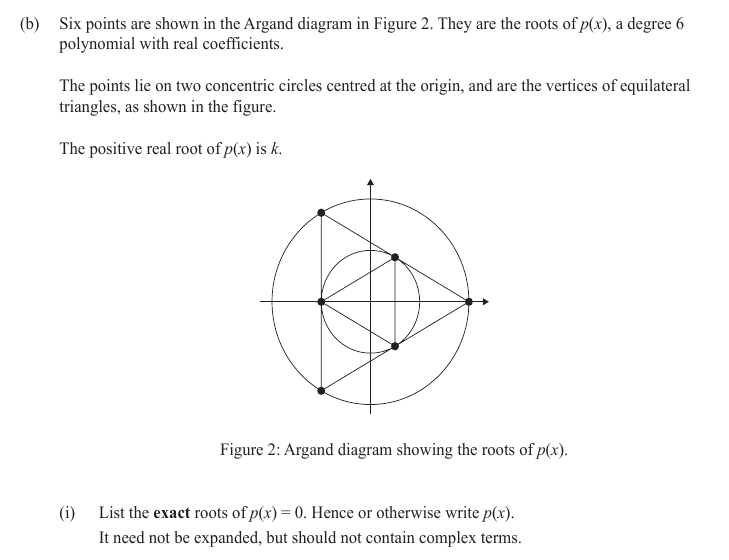
\includegraphics[width=\textwidth]{double_triangle}
\end{center}

The question states that the positive real solution is $ z_1 = k = k \cis 0 $. We
can therefore see that the other two solutions on the outer circle will be given
by $ z_2 = k \cis \frac{2\pi}{3} $ and $ z_3 = k \cis \frac{-2\pi}{3} $.

The negative real solution will have the same real part as the two complex solutions
on the outer circle; we can calculate this by taking $ z_4 = k \cos \frac{2\pi}{3} = -\frac{k}{2} $.
We can find the other two solutions on the inside circle by rotating our negative
real solution by $ \frac{2\pi}{3} $, obtaining $ z_5 = \frac{k}{2} \cis (\pi - \frac{2\pi}{3}) = \frac{k}{2} \cis \frac{\pi}{3} $
and $ z_6 = \frac{k}{2} \cis \frac{-\pi}{3} $.

\begin{center}
\begin{tabular} {c | c | c}
  \textbf{Root} & \textbf{Polar form} & \textbf{Rectangular form}\\
  $ z_1 $ & $ k \cis 0 $                         & $ k $\\
  $ z_2 $ & $ k \cis \frac{2\pi}{3} $            & $ -\frac{k}{2} + i\frac{k\sqrt{3}}{2} $\\
  $ z_3 $ & $ k \cis \frac{-2\pi}{3} $           & $ -\frac{k}{2} - i\frac{k\sqrt{3}}{2} $\\
  $ z_4 $ & $ \frac{k}{2} \cis \pi $             & $ -\frac{k}{2} $\\
  $ z_5 $ & $ \frac{k}{2} \cis \frac{\pi}{3} $   & $ \frac{k}{4} + i\frac{k\sqrt{3}}{4} $\\
  $ z_6 $ & $ \frac{k}{2} \cis \frac{-\pi}{3} $   & $ \frac{k}{4} - i\frac{k\sqrt{3}}{4} $\\
\end{tabular}
\end{center}

We now generate our polynomial using the techniques described in the section on
quadratic equations:
\begin{align*}
  f(x) &= (x - z_1)(x - z_4) = \left(x -k\right)\left(x + \frac{k}{2}\right)\\
  g(x) &= (x - z_2)(x - z_3) = \left(x - \left(-\frac{k}{2} + i\frac{k\sqrt{3}}{2}\right)\right)\left(x - \left(-\frac{k}{2} - i\frac{k\sqrt{3}}{2}\right)\right)\\
       &= x^2 - \frac{k}{2}x + \frac{k^2}{4}\\
  h(x) &= (x - z_5)(x - z_6) = \left(x - \left(\frac{k}{4} + i\frac{k\sqrt{3}}{4}\right)\right)\left(x - \left(\frac{k}{4} - i\frac{k\sqrt{3}}{4}\right)\right)\\
       &= x^2 + kx + k^2\\
  \therefore~p(x) &= f(x)g(x)h(x) = \left(x -k\right)\left(x + \frac{k}{2}\right)\left(x^2 - \frac{k}{2}x + \frac{k^2}{4}\right)\left(x^2 + kx + k^2\right)
\end{align*}

Note that because all of the complex roots come in conjugate pairs the imaginary parts
cancel leaving us with a sextic polynomial with real coefficients.

\begin{figure}
  \centering
  \begin{tikzpicture}
    \begin{axis}[
      xlabel=$x$,
      ylabel={$p(x)$ when $ k = 2 $},
      axis lines=middle
    ]
      \addplot[domain=-2.1:2.1, samples=100, color=WildStrawberry]{(x -2)*(x + (2/2))*(x^2 - (2/2)*x + (2^2)/4)*(x^2 + 2*x + 2^2)};
    \end{axis}
  \end{tikzpicture}
  \caption{A polynomial with the desired roots.}
\end{figure}

\subsection*{Exercises}
Work through the problem, writing out all working clearly. Attempt the problem without
looking at the solution. Describe the main ideas used in each step of the solution,
and make sure you understand why each step is taken and why the solution is correct.

Are there any other possible ways of completing the problem? Is this the only possible
solution?

\section{Solving the Cubic}\label{sec:cubic}
This section presents a general solution for the cubic equation similar to the solution
of the quadratic equation given in exercise \ref{sec:quadratic}.\ref{ex:quadratificational}. Be sure to complete that
exercise before reading this section. The general outline of this proof is given in \S14
of \cite{Edw84}.

\begin{figure}
  \centering
  \begin{minipage}{0.5\textwidth}
  \begin{center}
    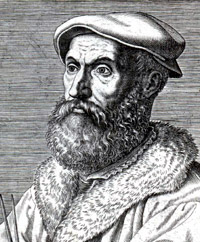
\includegraphics[width=0.4\linewidth]{tartaglia}
  \end{center}
  \end{minipage}%
  \begin{minipage}{0.5\textwidth}
  \begin{center}
    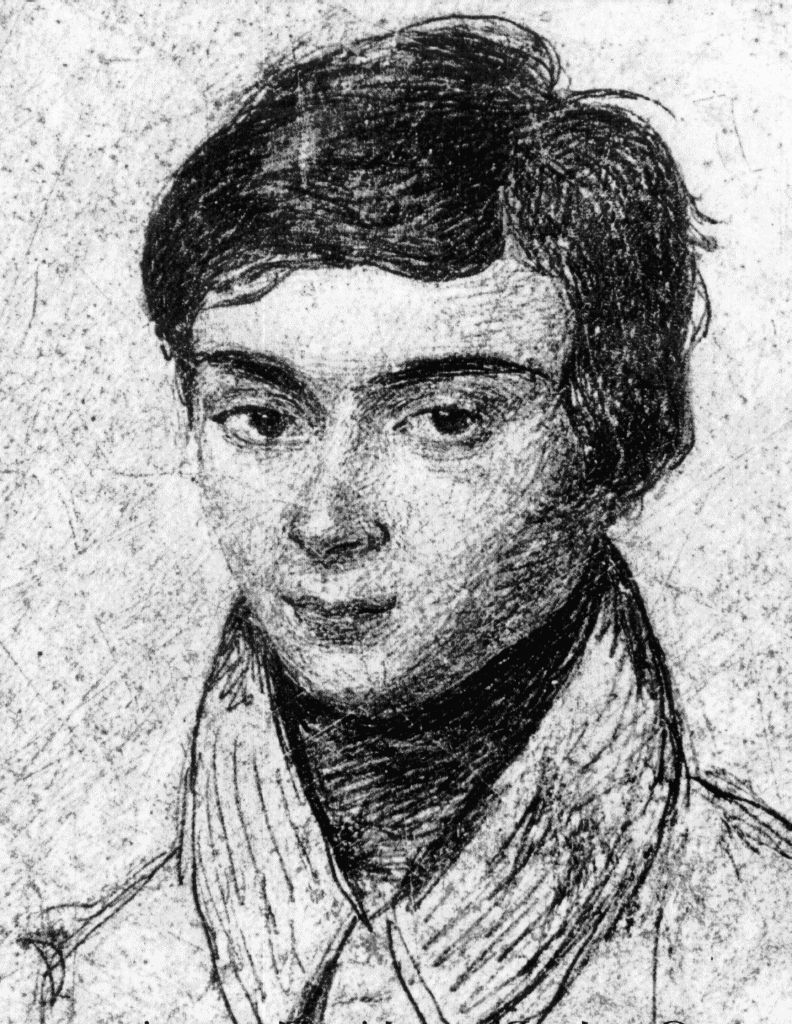
\includegraphics[width=0.4\linewidth]{galois}
  \end{center}
  \end{minipage}
  \caption{Niccolo Fontana (Tartaglia) (left) and \'Evariste Galois (right)}
\end{figure}

This particular method of solution was presented first by the French mathematician Alexandre-Th\'eophile Vandermonde
in 1771. However, it is believed that the first person to solve the general cubic equation was the Italian
Scipio de Ferro who passed on at least part of his method to his student Antonio Fior. A solution
was independently discovered at around the same time (in 1535) by Niccolo Fontana (also known as Tartaglia,
the Stammerer), who was conviced to pass them on to another Italian, Girolamo Cardano. Cardano later (in 1545)
published the solution in his book, \emph{Ars Magna}, which also included a solution to the general quartic
by Ludovico Ferrari.

Suppose we have some polynomial $ t^3 - \sigma_1 t^2 + \sigma_2 t - \sigma_3 $ (note the signs
on the coefficients) with the three complex roots (not necessarily distinct) $ x $, $ y $,
and $ z $. So $ \sigma_1 = x + y + z $, $ \sigma_2 = xy + xz + yz $, and $ \sigma_3 = xyz $,
where $ \sigma_n $ is known as the $ n$th elementary symmetric polynomial in $ x $, $ y $, and $ z $.

We note the following three identities:
\begin{align*}
  x^2z + xy^2 + yz^2 + x^2y + xz^2 + y^2z &= \sigma_1\sigma_2 - 3\sigma_3\\
  x^3 + y^3 + z^3 &= \sigma_1^3 - 3(\sigma_1\sigma_2 - 3\sigma_3) - 6\sigma_3\\
  x^2 + y^2 + z^2 &= \sigma_1^2 - 2\sigma_2
\end{align*}

Finally, let $ \alpha $ be a primitive cube root of 1.

\subsection*{Computations for the Solution}
Note first that
\begin{align*}
  x &= \frac{1}{3}\left( (x + y + z) + (x + \alpha y + \alpha^2 z) + (x + \alpha^2 y + \alpha z) \right)\\
    &= \frac{1}{3}\left( (x + y + z) + \sqrt[3]{(x + \alpha y + \alpha^2 z)^3} + \sqrt[3]{(x + \alpha^2 y + \alpha z)^3} \right)\\
    &= \frac{1}{3}\left( \sigma_1 + \sqrt[3]{(x + \alpha y + \alpha^2 z)^3} + \sqrt[3]{(x + \alpha^2 y + \alpha z)^3} \right)
\end{align*}
(remembering that the three cube roots of 1 add to 0).

Now, we must find expressions for $ u = (x + \alpha y + \alpha^2 z)^3 $ and $ v = (x + \alpha^2 y + \alpha z)^3 $ in terms of
the coefficients of the polynomial, $ \sigma_n $. Suppose that we can find $ uv $ and $ u + v $ in terms of the elementary
symmetric polynomials. Then we can find $ u $ and $ v $ using the quadratic formula.

So what are $ uv $ and $ u + v $?

Expanding $ u $ and $ v $ individually, we find
\begin{align*}
  u &= 3(x^2z + xy^2 + yz^2)\alpha^2 + 3(x^2y + xz^2 + y^2z)\alpha + x^3 + y^3 + z^3 + 6xyz, \text{ and}\\
  v &= 3(x^2z + xy^2 + yz^2)\alpha + 3(x^2y + xz^2 + y^2z)\alpha^2 + x^3 + y^3 + z^3 + 6xyz.
\end{align*}

Adding these together, we have
\begin{align*}
  u + v &= &&  3\alpha(x^2z + xy^2 + yz^2 + x^2y + xz^2 + y^2z)\\
        &  &&+ 3\alpha^2(x^2z + xy^2 + yz^2 + x^2y + xz^2 + y^2z)\\
        &  &&+ 12xyz + 2(x^3 + y^3 + z^3)\\
        &= &&3(\alpha + \alpha^2)(\sigma_1\sigma_2 - 3\sigma_3) + 12\sigma_3 + 2(\sigma_1^3 - 3(\sigma_1\sigma_2 - 3\sigma_3) - 6\sigma_3)\\
        &= &&-3(\sigma_1\sigma_2 - 3\sigma_3) + 12\sigma_3 + 2(\sigma_1^3 - 3(\sigma_1\sigma_2 - 3\sigma_3) - 6\sigma_3)\\
        &= &&2\sigma_1^3 - 9\sigma_1\sigma_2 + 27\sigma_3.
\end{align*}

To find $ uv $, we proceed as follows:
\begin{align*}
  (x + \alpha y + \alpha^2 z)(x + \alpha^2 y + \alpha z) &= (xy + xz + yz)\alpha^2 + (xy + xz + yz)\alpha + x^2 + y^2 + z^2\\
                                                         &= (\alpha + \alpha^2)(\sigma_2) + \sigma_1^2 - 2\sigma_2\\
                                                         &= \sigma_1^2 - 3\sigma_2\\
                                                         &\Downarrow\\
                                                      uv &= (\sigma_1^2 - 3\sigma_2)^3.
\end{align*}

\subsection*{Solution}
So, to find the solutions of a cubic equation $ t^3 - \sigma_1 t^2 + \sigma_2 t - \sigma_3 = 0 $:
\begin{enumerate}
  \item Calculate:
    \begin{align*}
      u + v &= 2\sigma_1^3 - 9\sigma_1\sigma_2 + 27\sigma_3\\
      uv    &= (\sigma_1^2 - 3\sigma_2)^3
    \end{align*}
  \item Then calculate:
    \begin{displaymath}
      u,v = \frac{(u+v) \pm \sqrt{(u  + v)^2 - 4uv}}{2}
    \end{displaymath}
  \item Hence, we have nine possible solutions (one for each choice of cube root), of
        which three will work in the original equation (trial and error must be used at this point):
    \begin{align*}
      x &= \frac{1}{3}\left( \sigma_1 + \sqrt[3]{u} + \sqrt[3]{v} \right)
    \end{align*}
    Remember that the three cube roots of a number will be $ \sqrt[3]{u} $, $ \alpha\sqrt[3]{u} $,
    and $ \alpha^2 \sqrt[3]{u} $ where $ \alpha $ is a complex cube root of unity.
\end{enumerate}

A variation of this method also solves quartic equations. However, no general solution to the
quintic equation (or any higher degree equation) exists in terms of radicals (terms under a $ \sqrt{} $).
The lack of a general solution for any polynomial with $ \delta > 5 $ was originally proved by Ruffini
and Abel in the early 1800s, and a general study of the symmetries of the roots of polynomials
(the beginnings of Galois theory) was first published (after being rejected twice) by the
French Academy of Sciences in 1843 after their late author \'Evariste Galois was killed in a duel
over a girl in 1832 (at the age of 20). For more historical details, see the introductory chapter
of \cite{Ste15}.

\subsection*{Clearing Up Some Technical Points}
How did we know that $ uv $ and $ u + v $ could be expressed in terms of the elementary
symmetric polynomials (the coefficients)? Well, it so happens that $ uv $ and $ u + v $ are
symmetric in $ x $, $ y $, and $ z $ (this is not hard to check), and we have a theorem due
to Sir Isaac Newton which states that:
\begin{thm}[Fundamental Theorem on Symmetric Polynomials]
  Suppose that $ r_1 $, $ r_2 $, ..., $ r_n $ are the roots of some polynomial. Then every
  symmetric polynomial in $ r_1 $, $ r_2 $, ..., $ r_n $ can be expressed (uniquely) as a polynomial
  in the elementary symmetric functions $ \sigma_1 $, $ \sigma_2 $, ..., $ \sigma_n $.
\end{thm}
Note that the elementary symmetric functions of order $ n $ are simply the coefficients of
the polynomial $ (x - a_1)(x - a_2) \cdots (x - a_n) $. For example, the second-order elementary
symmetric functions are just $ \sigma_1 = a_1 + a_2 $ and $ \sigma_2 = a_1 a_2 $; the third-order
elementary symmetric functions are just $ \sigma_1 = a_1 + a_2 + a_3 $, $ \sigma_2 = a_1 a_2 + a_1 a_3 + a_2 a_3 $,
and $ \sigma_3 = a_1 a_2 a_3 $.

Basically, the theorem implies that if we have a symmetric expression in the roots of some polynomial,
then we can write that expression in terms of the coefficients of the polynomial.

One example is the discriminant of a polynomial. We have already met the discriminant of a quadratic, $ \Delta_2 = b^2 - 4ac $;
we can more generally define the discriminant of an $ n$th degree polynomial to be
\begin{displaymath}
\Delta_n [(x - \alpha_1)(x - \alpha_2) \cdots (x - \alpha_n)] = \prod_{i < j}(\alpha_i - \alpha_j)^2
\end{displaymath}
which is obviously symmetric in each $ \alpha_i $.

\subsection*{Exercises}
\begin{enumerate}
  \harder Check the author's algebra.
  \item Solve $ t^3 + t^2 - 89t + 231 = 0 $.
  \item Solve $ t^3 + 21t^2 - 32t + 3510 = 0 $.
  \item Solve $ 2t^3 + 4i t^2 + 58t - 84i = 0 $.
  \item In 1225, Leonardo of Pisa (Fibonacci) was asked by Holy Roman Emperor Frederick II
        to solve the cubic equation $ x^3 + 2x^2 + 10x = 20 $. His solution was
        \begin{displaymath}
          x = 1 + \frac{22}{60} + \frac{7}{60^2} + \frac{42}{60^3} + \frac{33}{60^4} + \frac{4}{60^5} + \frac{40}{60^6}.
        \end{displaymath}
        \begin{enumerate}
          \item Show that the equation has exactly one real root.
          \item Use the method outlined in this section to find numerical approximations to the three roots
                of the polynomial.
        \end{enumerate}
  \item Solve $ t^3 - 15t - 4 = 0 $ using the methods outlined in this section. See exercise \ref{ex:cardano}
        from the section on complex numbers.
  \item Verify that $ uv $ and $ u + v $ are symmetric in $ x $, $ y $, and $ z $.
  \item Read the historical introduction of Ian Stewart's \textit{Galois Theory} \cite{Ste15}.
  \item The discriminant of the general quartic equation $ q(x) = A(x - \alpha)(x - \beta)(x - \gamma)(x - \delta) $ is
        given by the formula
        \begin{displaymath}
          \Delta_4 [q(x)] = (\alpha - \beta)^2(\alpha - \gamma)^2(\alpha - \delta)^2(\beta - \gamma)^2(\beta - \delta)^2(\gamma - \delta)^2.
        \end{displaymath}
        Suppose that for a particular quartic $ Q(x) $ with real coefficients, $ \Delta_4[Q(x)] > 0 $. What can you say about the number of real roots?
\end{enumerate}

\section{Final Exercises}\label{sec:finalexs}

\begin{aquote}{Jacques Hadamard}
  The shortest path between two truths in the real domain passes through the complex domain.
\end{aquote}

These exercises broadly cover the content of the book, and their difficulty
varies! However, in general it is a good idea to look at the exercises in each
section first as they often include some content themselves.

\begin{enumerate}
  \item Is $ (x-15) $ a factor of $ (x^3 - 19x - 30) $? Is $ (x^2 + 5x + 6) $ a factor?
  \item Factor completely $ 9x^4 - 13x^2 + 4 $.
  \item Solve $ x^3 + 9x^2 = 60 - 8x $.
  \item Find $ k $ such that $ (x - 4) $ is a factor of $ x^3 + 7x^2 - 14x + k $.
  \item Find a value of $ k \neq 0 $ such that $ kx^2 -6x + 1 = 0 $ will have just one root.
  \item Find all sixth roots of $ i $.
  \item Find $ k $ such that $ 8 - x +  2\sqrt{2x + k} = 0 $ has exactly one real root.
  \item Solve $ (\alpha^2 + 2\alpha -4)(\alpha^7 + 1) = 0 $.
  \item Solve $ x^4 + x^2 + 1 = 0 $ for $ x $.
  \hard Solve $ \beta^2 + \beta + 1 = 0 $ for $ x $ if $ \beta = x^2 + x + 1 $.
  \hard Let $ \alpha $, $ \beta $, and $ \gamma $ be the three roots of $ ax^3 + bx^2 + cx + d = 0 $. Prove that:
        \begin{enumerate*}
          \item $ \alpha + \beta + \gamma = \frac{-b}{a} $,
          \item $ \alpha\beta + \beta\gamma + \alpha\gamma = \frac{c}{a} $, and
          \item $ \alpha\beta\gamma = \frac{-d}{a} $.
        \end{enumerate*}
        Hence show that $ \alpha^2\beta\gamma + \alpha\beta^2\gamma + \alpha\beta\gamma^2 = \frac{bd}{a^2} $.
  \item Solve $ (z+1)^3 = 8(z-1)^3 $ for $ z $. Give exact answers in the form $ a + ib $.
  \item Graph the equation $ \abs{z} = 3 $ in the complex plane.
  \item If $ z = 1+i $ and $ w = \frac{1}{z} + i $, find the argument of $ w $.
  \hard If $ \frac{z + 2i}{z-2i} $ is purely imaginary, describe the possible values of $ z $.
  \item If $ \abs{z - 1 + 2i} = \abs{z + 1} $ and $ z = x+yi $, find an expression for $ y $ in terms
        of $ x $ (i.e. find the locus of $ z $).
  \item Sketch the region satisfied by $ \realp{z - i \overline z} > 2 $.
  \item If $ x = 2 $ and $ x = 6 $ are solutions of $ p(x) = Ax^2 + Bx + C $ and $ p(0) = -4 $,
        find $ A $, $ B $, and $ C $.
  \item If $ w = 2-3i $ is a zero of $ 3w^3 - 14w^2 + Aw - 26 $ (where $ A $ is real), find $ A $
        and the remaining two roots.
  \hard Use de Moivre's Theorem to show that
        \begin{enumerate}
          \item $ \sin 2\theta = 2\sin\theta\cos\theta $ and $ \cos 2\theta = \cos^2 \theta - \sin^2 \theta $; and
          \item $ \sin 3\theta = 3\sin\theta - 4\sin^3\theta $ and $ \cos 3\theta = 4\cos^3\theta - 3\cos\theta $.
        \end{enumerate}
  \item Use Euler's formula to prove that $ \cos(\alpha + \beta) = \cos \alpha \cos \beta - \sin \alpha \sin \beta $, and that
        $ \sin(\alpha + \beta) = \sin \alpha \cos \beta + \cos \alpha \sin \beta $.
  \harder Show that $ \arctan a + \arctan b = \arctan \frac{a + b}{1 - ab} $.
  \hard Suppose that $ \abs{z+w} = \abs{z-w} $. Show that $ \carg z - \carg w = \pm \frac{\pi}{2} $.
  \hard If $ 3z^3 + (2-3ai)z^2 + (6+2bi)z + 4 $ has exactly one real root, what value must
        the quotient $ b/a $ take if both $ a $ and $ b $ are real? Find the real root.
  \hard Find all possible values for $ \theta $ if $ \cis^2 \theta + \cis \theta + 1 = 0 $.
  \item Graph the locus of $ \carg w = \abs{w} $. What about $ \carg w + \abs {w} = 1 $?
  \item Given a quadratic equation $ x^2 + px + q $ and a root $ \alpha $, show that the other root $ \beta $ is
        given by $ \beta = -p - \alpha $ and find a similar expression for finding two roots of a cubic given the
        third.
  \item Suppose $ p $ is a quadratic (i.e. $ p(x) = ax^2 + bx + c $ for some $ a $, $ b $, and $ c $). Suppose further
        that $ p(0) = 9 $, and $ p(3) = 0 $. How many distinct roots does $ p $ have?
  \hard Use the identity $ x^2 + y^2 = (x-iy)(x+iy) $ to prove that if $ m $ and $ n $ are integers that can be written as the sum of two
        squares, then their product $ mn $ can also be written as a sum of two squares.
  \item Solve the following system of equations:
        \begin{align*}
          x^2 + 4xy + y^2 &= 2\\
          x^2 - 2xy + y^2 &= -4
        \end{align*}
  \item Suppose $ \omega $ is a primitive cube root of unity. Show that
        \begin{displaymath}
          y_2 = \omega \sqrt[3]{\frac{1}{2}(-1 + \sqrt{5})} + \omega^2 \sqrt[3]{\frac{1}{2}(-1 - \sqrt{5})}
        \end{displaymath}
        and
        \begin{displaymath}
          y_3 = \omega^2 \sqrt[3]{\frac{1}{2}(-1 + \sqrt{5})} + \omega \sqrt[3]{\frac{1}{2}(-1 - \sqrt{5})}
        \end{displaymath}
        are complex conjugates.
  \item Find all solutions to $ x^{n - 1} + x^{n - 2} + \cdots + 1 = 0 $, where $ n $ is a natural number.
  \item \label{ex:solutiongenerator}
    \begin{enumerate}
      \item Let $ p(x) = \sum^n_{r = 0} p_r x^r $ be a polynomial with real coefficients. If $ p(z) = 0 $,
            then $ p(\overline{z}) = 0 $. (This is a generalisation of \ref{sec:complex1}.\ref{ex:conjquadratic} to arbitrary degree polynomials.)
      \item Let $ p(x) = \sum^n_{r = 0} p_r x^{2r} $ be a polynomial with real coefficients and only even powers of $ x $.
            If $ p(a + bi) = 0 $, then $ p(\pm a \pm bi) = 0 $ for all possible combinations of $ \pm $.
    \end{enumerate}
  \hard Under which conditions will the equation $ x^2 + a(1+i)x + b(1+i) = 0 $ have one or more
        real solutions if both $ a $ and $ b $ are real?
  \item Find the complex number $ z $ which satisfies $ \carg(z - 1 - i) = -\frac{\pi}{6} $ and
        $ \carg(z - 1 + i) = \frac{\pi}{6} $.
  \harder Find all integer values of $ a $ and $ b $ such that $ \frac{a^2+b^2}{ab} $ is an integer.
  \harder Let $ w $ and $ z $ be complex numbers, and let $ u = w + z $ and $ v = w^2 + z^2 $. Prove
          that $ w $ and $ z $ are real \textbf{if and only if} $ u $ and $ v $ are real and $ u^2 \leq 2v$.
  \hard Suppose $ x + \frac{1}{x} = 1 $.
        \begin{enumerate}
          \item Show, without calculating $ x $, that we must necessarily have
            \begin{displaymath}
              x^7 + \frac{1}{x^7} = 1
            \end{displaymath}
          \item Calculate the possible values of $ x $ and verify this fact.
        \end{enumerate}
  \harder Calculate $ i^i $.
  \item Let $ \mathbb{R}[\epsilon] $ be the real numbers together with some new element $ \epsilon \neq 0 $ such that $ \epsilon^2 = 0 $.
        \begin{enumerate}
          \item Does there exist $ \beta $ in $ \mathbb{R}[\epsilon] $ such that $ \beta \epsilon = 1 $ (i.e. does $ \epsilon $ have a multiplicative
                inverse)?
          \item When does $ (a + b\epsilon)^{-1} $ exist?
          \item Solve $ x^2 - 1 = 2\epsilon $ in $ \mathbb{R}[\epsilon] $.
        \end{enumerate}
  \hard Suppose $ p(x) = \sum_{i = 0}^n a_i x^i $ and $ q(x) = \sum_{i = 0}^m b_i x^i $ are polynomials. Show that
        \begin{displaymath}
          p(x) q(x) = \sum_{i = 0}^{m + n} c_i x^i,
        \end{displaymath}
        where each $ c_i $ is a constant. Give an expression for $ c_i $ in terms of the coefficients of $ p(x) $ and $ q(x) $.
  \harder In this exercise, we will prove the division theorem that we stated without proof in section \ref{section:poly}: if $ f $ and $ g \neq 0 $
          are polynomials, then there exist unique polynomials $ q $ and $ r $ such that $ \partial r < \partial g $ and
          \begin{displaymath}
            f(x) = g(x) q(x) + r(x).
          \end{displaymath}
    \begin{enumerate}
      \item Consider the set $ S $ of all polynomials of the form $ f(x) - g(x) q(x) $ for some polynomial $ q(x) $. Show that $ S $ is non-empty
            (i.e. exhibit some polynomial in $ S $).
      \item Explain why there must be some polynomial in $ S $ with minimal degree (that is, you cannot exhibit an infinite sequence of
            polynomials $ p_1, p_2, ... $ in $ S $ such that $ \partial p_1 > \partial p_2 > \cdots > \partial p_i > \cdots $).
      \item Pick such a polynomial of minimal degree; call it $ r $. Fix also the associated $ q $ (i.e. now we have $ f(x) = g(x) q(x) + r(x) $ for
            our fixed $ r $ and $ q $). Show that if $ \partial r \geq \partial g $, then it is possible to construct another polynomial in $ S $ with
            lower degree than $ r $. Conclude that $ \partial r < \partial g $.
      \item Show that $ q $ and $ r $ are uniquely determined by $ f $ and $ g $.
    \end{enumerate}
  \item Take the polynomial $ x^2 = 4 $ in the integers modulo 6 (i.e. the integers 0, 1, 2, 3, 4, 5
        such that $ 5 + 1 = 0 $). Solve for all possible values of $ x $.
  \item \textbf{Bonus exercise I:} In general, what numbers will work in the place of $ 3 $ and $ 9 $ in the XKCD
        comic at the bottom of the bibliography?
  \item \textbf{Bonus exercise II:} Notice that $ \frac{3}{16} - \frac{3}{19} = \frac{3}{16} \cdot \frac{3}{19} $.
        For which values of $ a $, $ b $, and $ d $ is the identity $ \frac{a}{b} - \frac{a}{d} = \frac{a}{b} \cdot \frac{a}{d} $ true?
\end{enumerate}

% \newpage\null\thispagestyle{empty}
\newpage
\nocite{*}
\printbibliography[title=Bibliography and Further Reading, heading=bibnumbered]

With thanks to Heydin Leeet for highlighting a typo in an exercise.

\vspace{\fill}

\begin{center}
  How to solve problems\\
  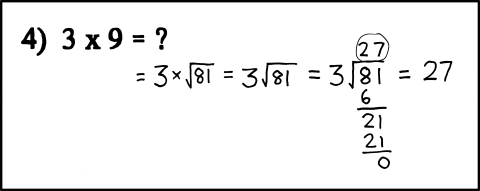
\includegraphics[width=0.5\textwidth]{3x9}\\
  \small{\textit{Image from \url{http://xkcd.com/759/}, CC BY-NC 2.5}}
\end{center}

\end{document}
